\appendix{Other results}\label{app:results}
All remaining results are in this section. 

%%%%%%%%%%%%%%%%%%%%%%%%%%%%%%%%%%%%%%%%%%%%%%%%%
%Chapter 4 Results
%%%%%%%%%%%%%%%%%%%%%%%%%%%%%%%%%%%%%%%%%%%%%%%%

%MASE

\begin{figure}[!ht]
	\begin{center}
		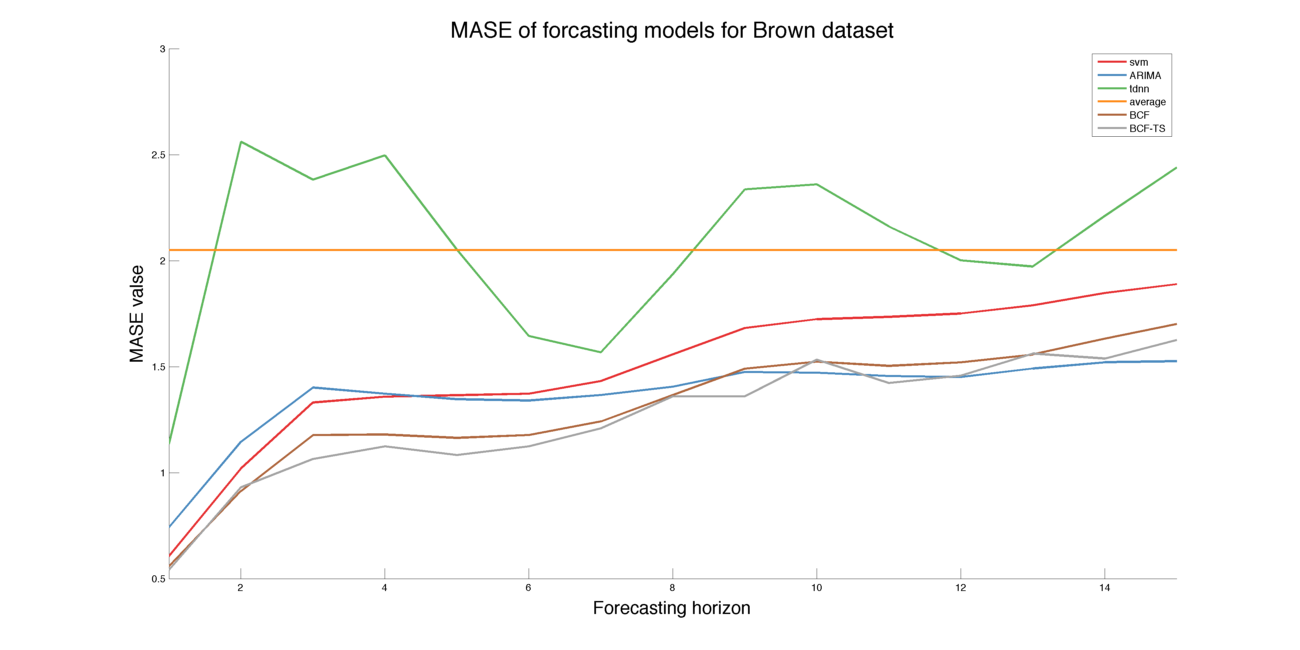
\includegraphics[width=1.0\linewidth]{mase_for_bcf-ts_for_Brown.png}
	\end{center}
	\caption{Brown dataset: Root mean square error of forecasting for each model vs forecasting horizon.}
	\label{fig:rmseplotbrown}
\end{figure}


\begin{figure}[!ht]
	\begin{center}
		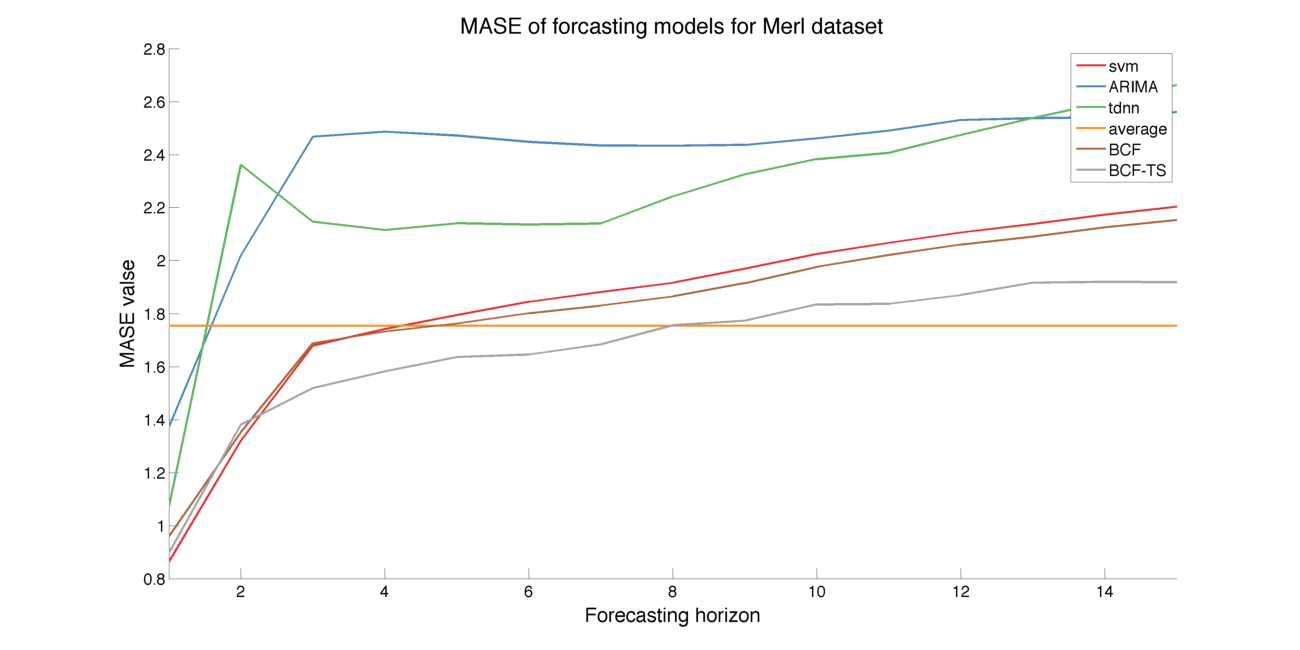
\includegraphics[width=1.0\linewidth]{mase_for_bcf-ts_for_Merl.png}
	\end{center}
	\caption{Merl dataset: root mean square error of forecasting for each model vs forecasting horizon.}
	\label{fig:maseplotmerl}
\end{figure}

\begin{figure}[!ht]
	\begin{center}
		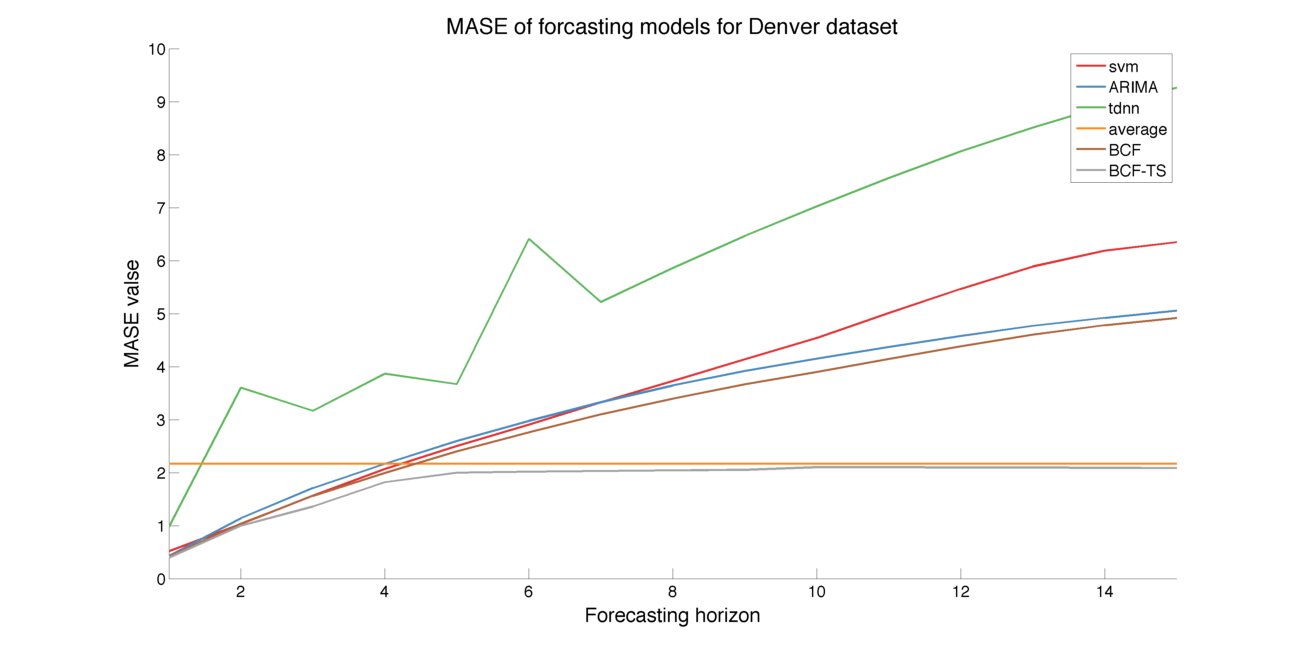
\includegraphics[width=1.0\linewidth]{mase_for_bcf-ts_for_Denver.png}
	\end{center}
	\caption{Denver dataset: root mean square error of forecasting for each model vs forecasting horizon.}
	\label{fig:maseplotdenver}
\end{figure}

%MASE Percent improvement
\begin{figure}[!ht]
	\begin{center}
		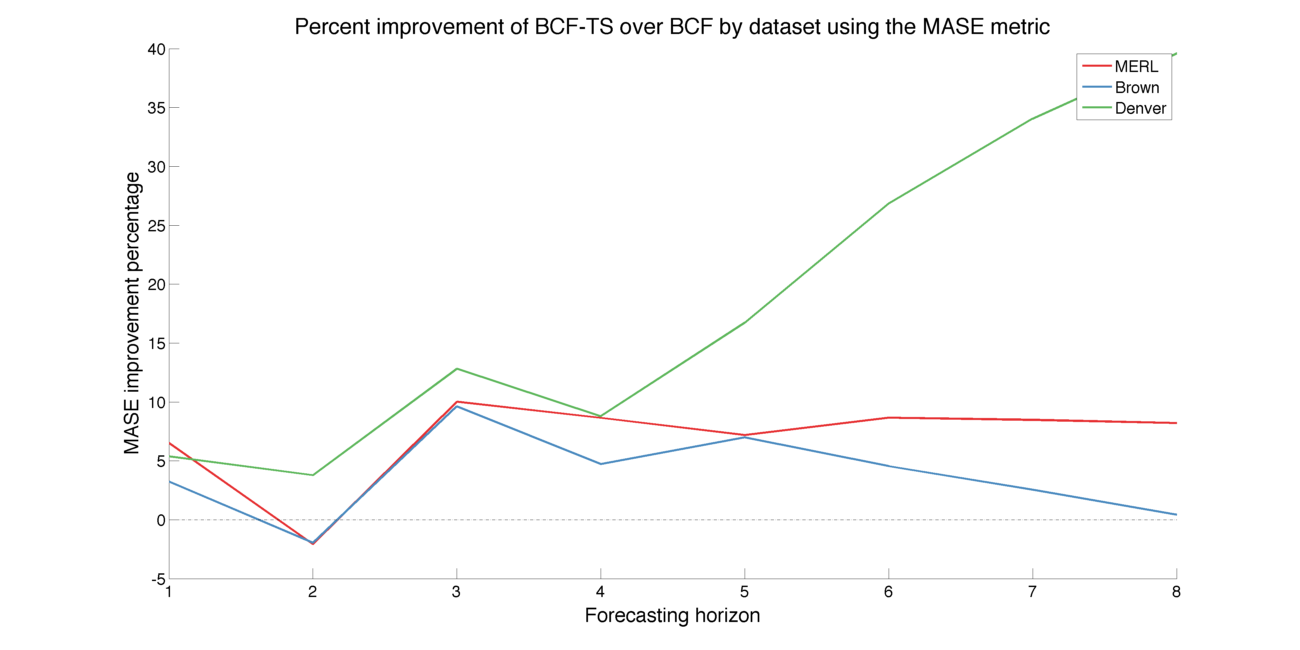
\includegraphics[width=1.0\linewidth]{BCF-TS_mase_improvement_for_each_dataset.png}
	\end{center}
	\caption{Improvement percentage of MASE values of BCF-TS compared to BCF.}
	\label{fig:bcftsmaseimprovement}
\end{figure}


%%%%%%%%%%%%%%%%%%%%%%%%%%%%%%%%%%%%%%%%%%%%%%%%%
%SQE Results per forecaster
%%%%%%%%%%%%%%%%%%%%%%%%%%%%%%%%%%%%%%%%%%%%%%%%%
%merl
\begin{figure}[!h]
	\begin{center}
		\subfigure[] {
			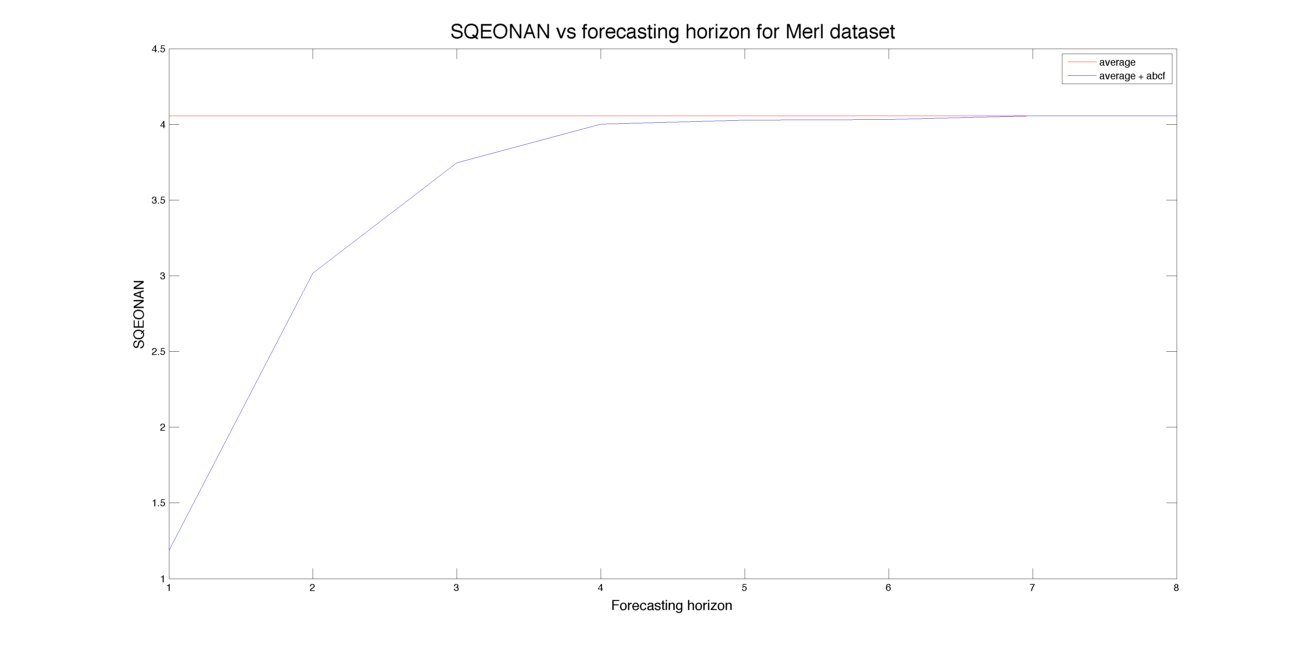
\includegraphics[width=0.4\textwidth]{sqe_merl_avg.png}
		}
		\subfigure[] {
			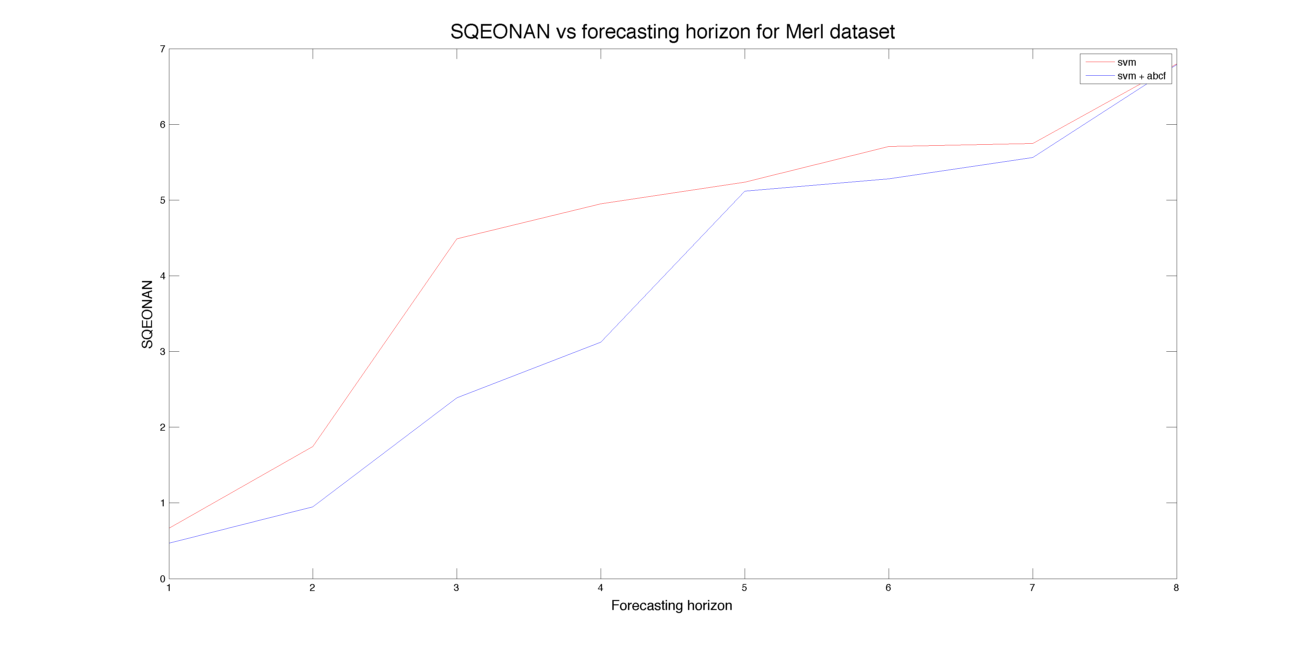
\includegraphics[width=0.4\textwidth]{sqe_merl_svm.png}
		} \\
		\subfigure[] {
			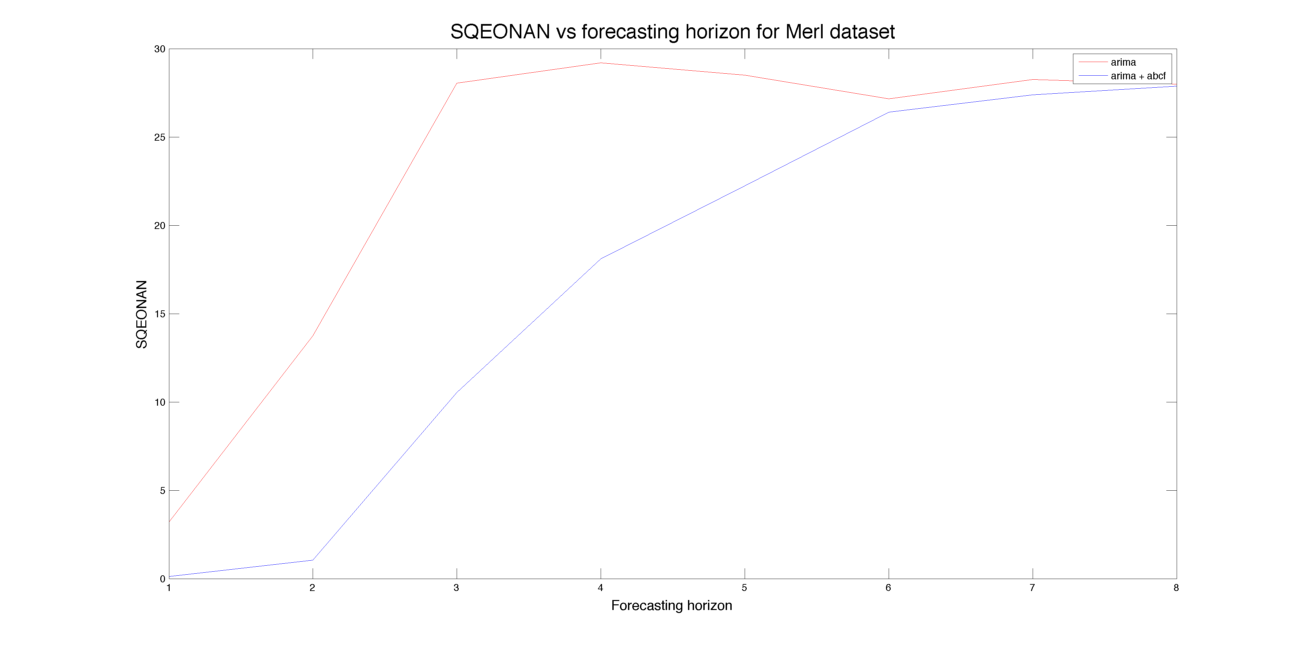
\includegraphics[width=0.4\textwidth]{sqe_merl_arima.png}
		}
		\subfigure[] {
			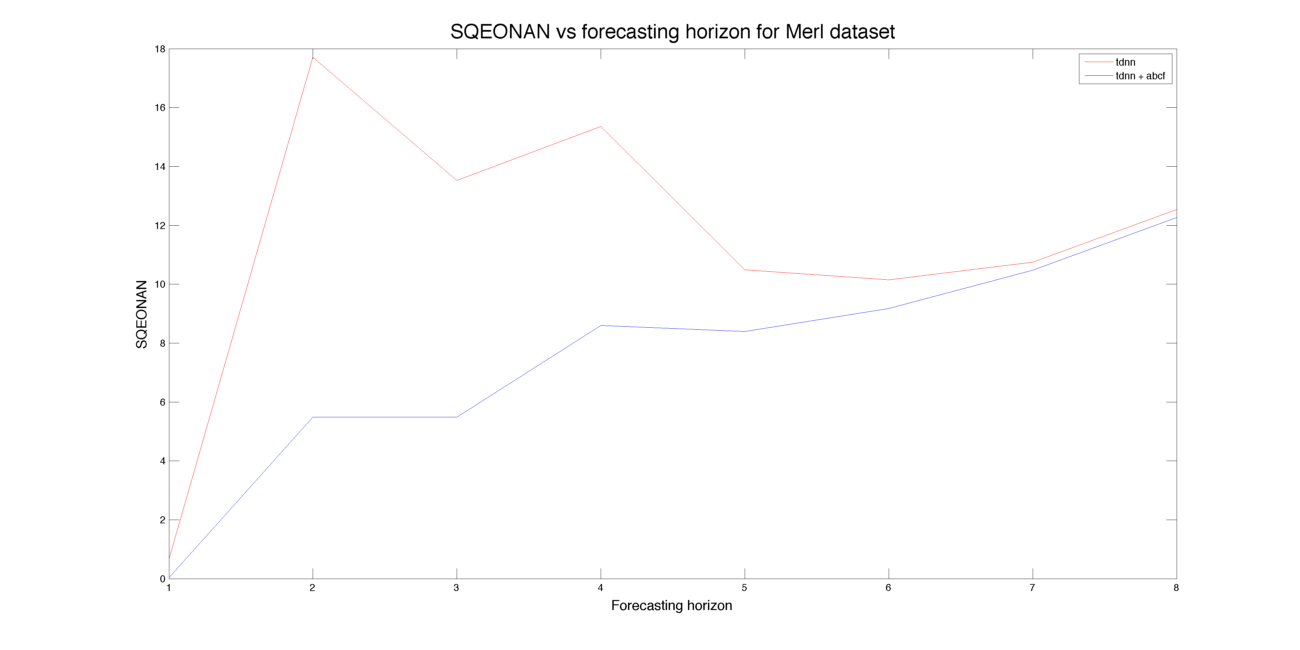
\includegraphics[width=0.4\textwidth]{sqe_merl_tdnn.png}
		}
	\end{center}
	\caption{Results for the four base forecasting algorithms for the Brown Hall dataset and the improvements to SQEONAN from using our ABCF algorithm}
	\label{fig:sqe_merl_results}
\end{figure}

%brown
\begin{figure}[!t]
	\begin{center}
		\subfigure[] {
			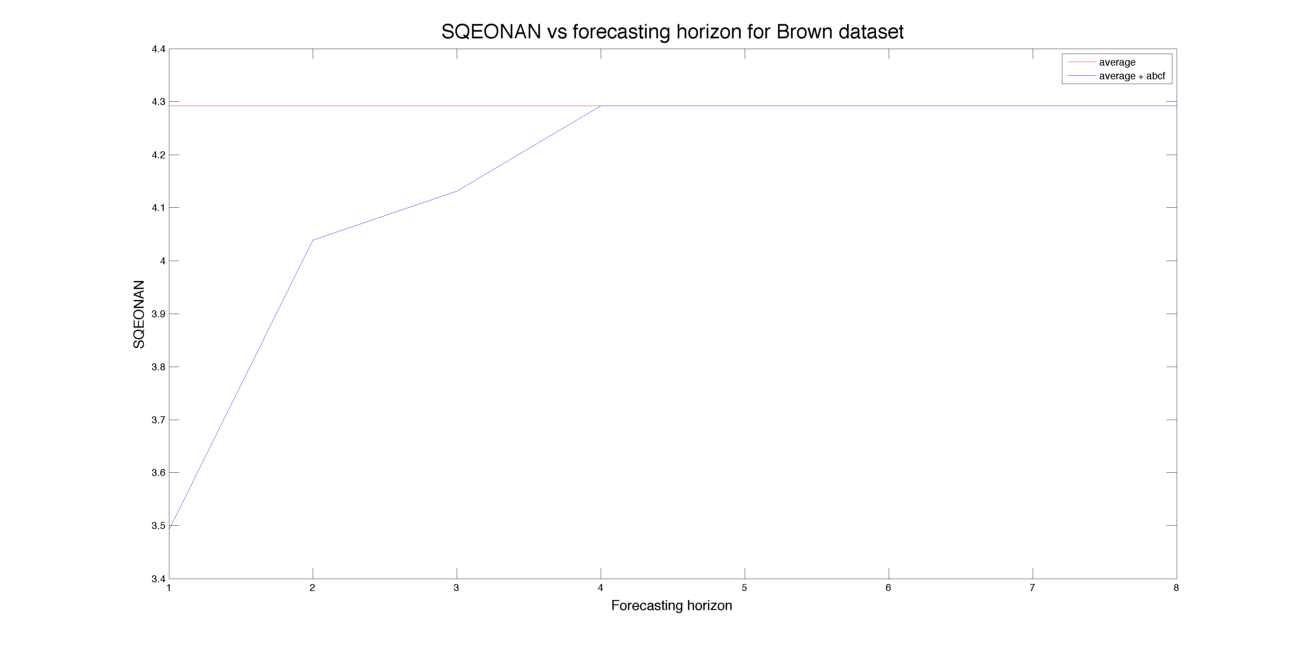
\includegraphics[width=0.4\textwidth]{sqe_brown_avg.png}
		}
		\subfigure[] {
			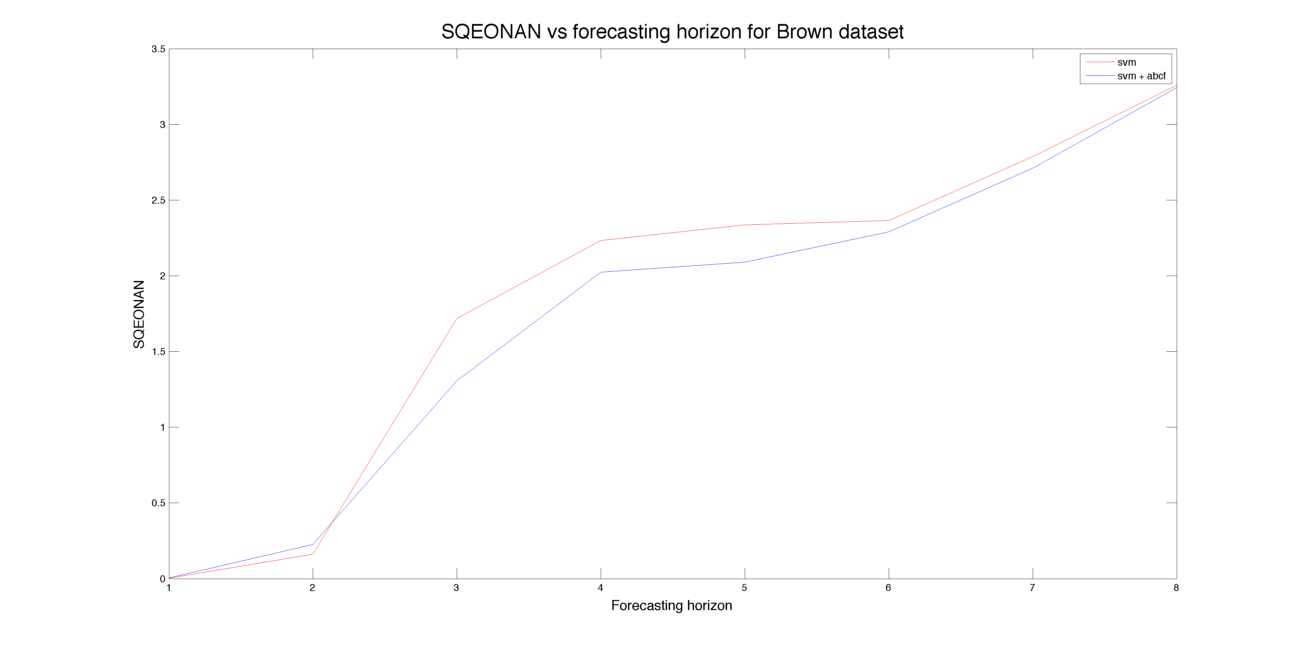
\includegraphics[width=0.4\textwidth]{sqe_brown_svm.png}
		} \\
		\subfigure[] {
			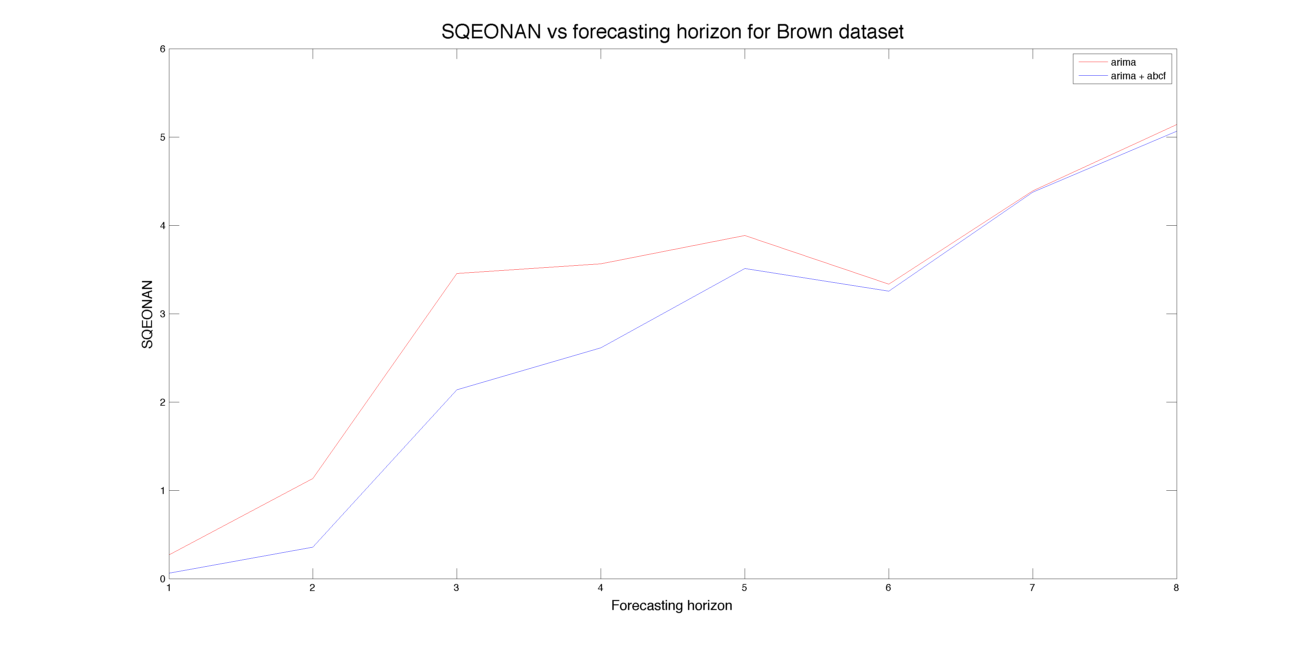
\includegraphics[width=0.4\textwidth]{sqe_brown_arima.png}
		}
		\subfigure[] {
			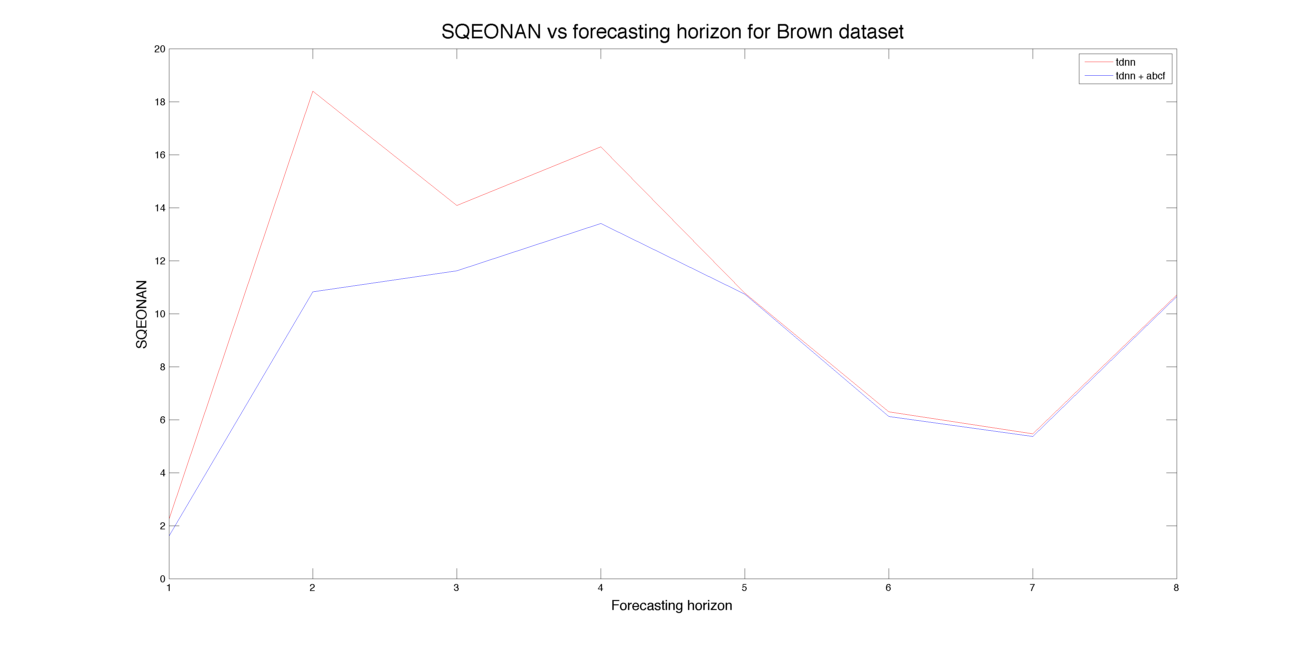
\includegraphics[width=0.4\textwidth]{sqe_brown_tdnn.png}
		}
	\end{center}
	\caption{Results for the four base forecasting algorithms for the Brown Hall dataset and the improvements to SQEONAN from using our ABCF algorithm}
	\label{fig:sqe_brown_results}
\end{figure}

%denver
\begin{figure}[!b]
	\begin{center}
		\subfigure[] {
			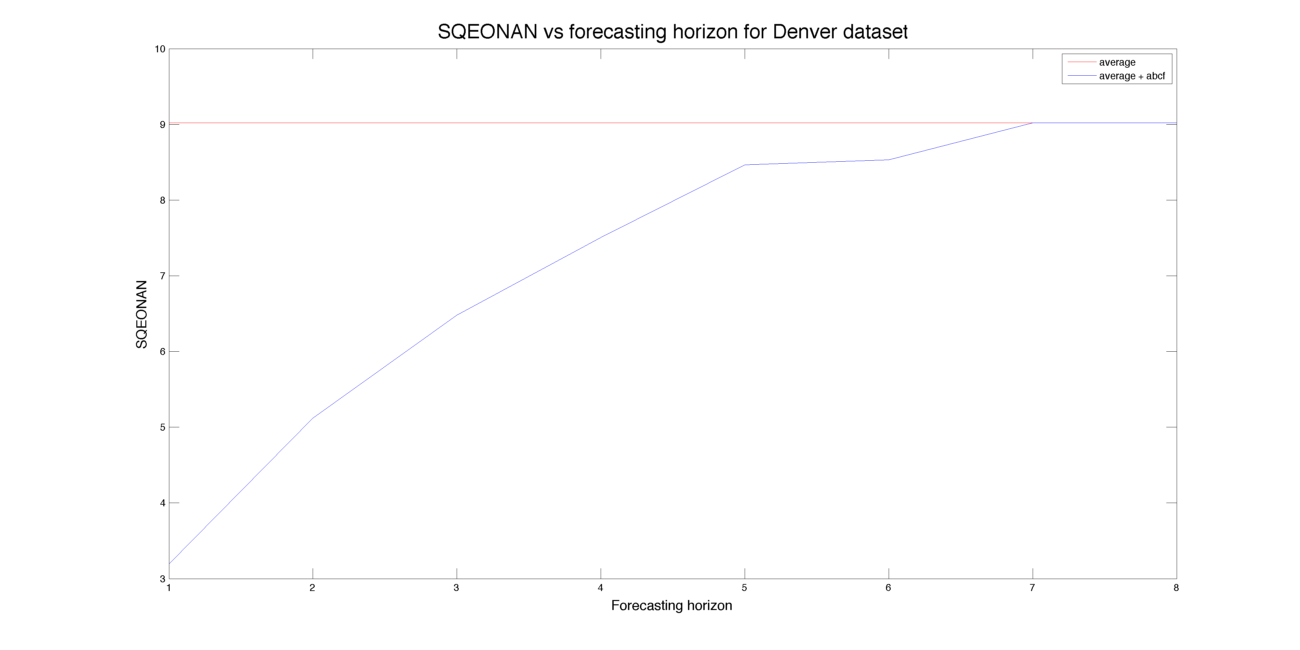
\includegraphics[width=0.4\textwidth]{sqe_denver_avg.png}
		}
		\subfigure[] {
			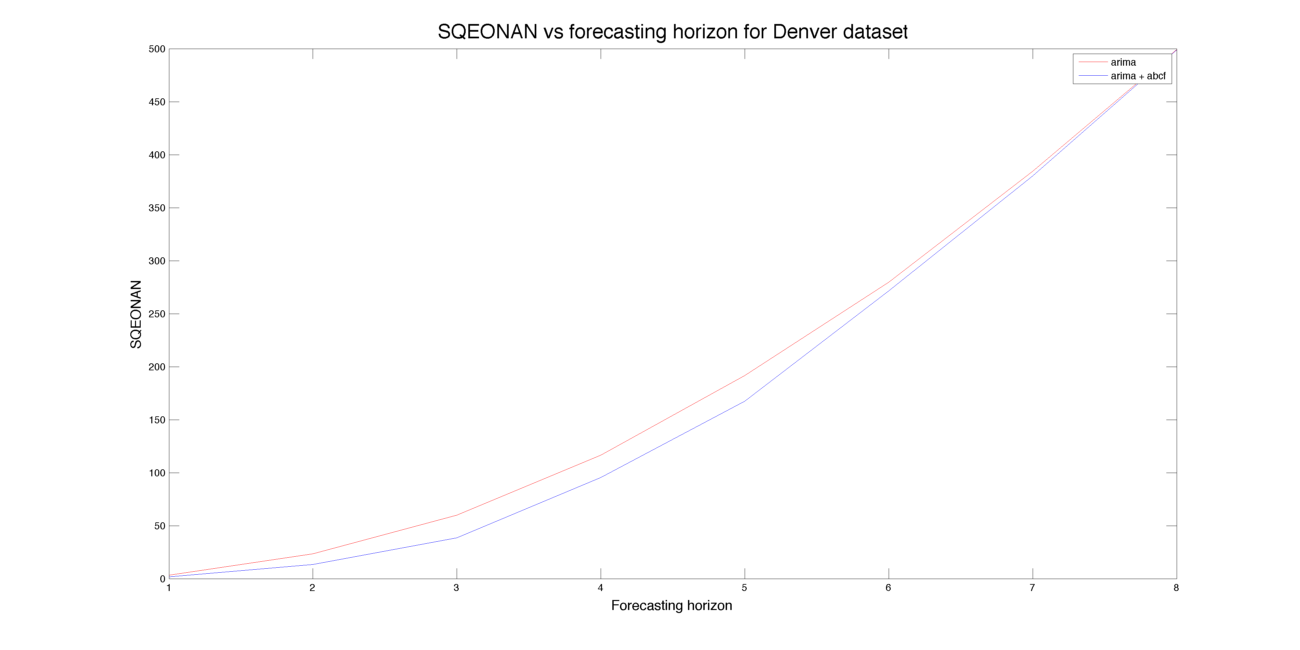
\includegraphics[width=0.4\textwidth]{sqe_denver_svm.png}
		} \\
		\subfigure[] {
			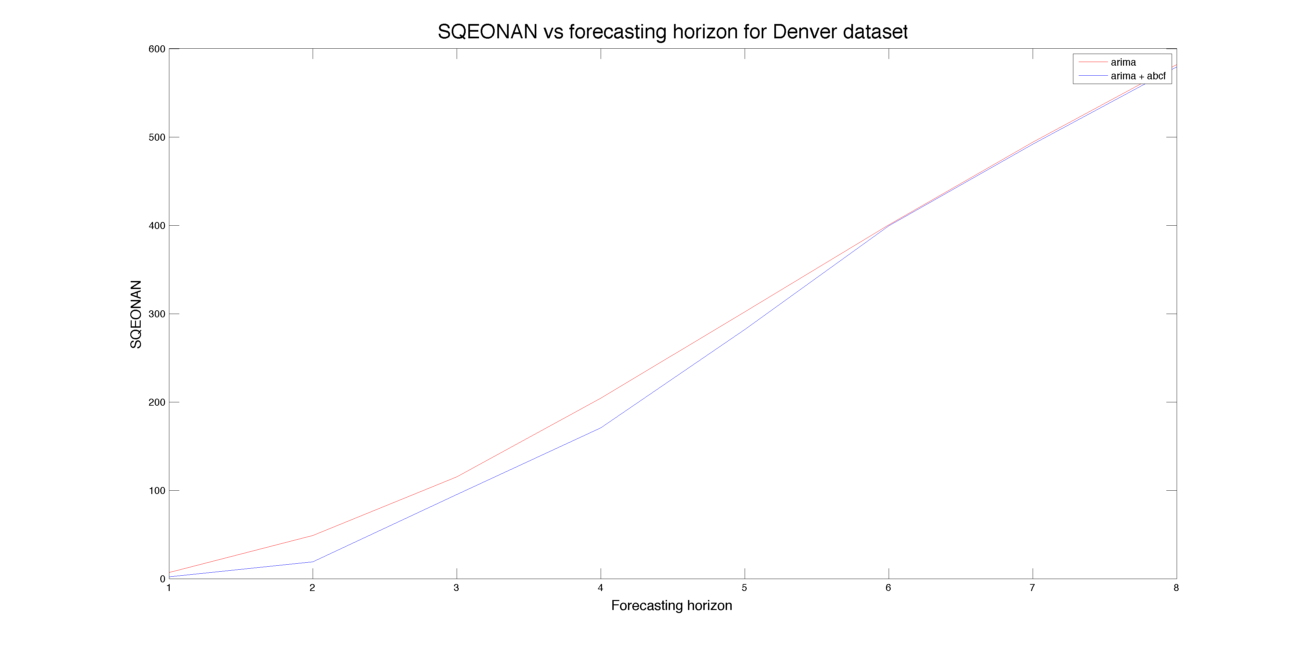
\includegraphics[width=0.4\textwidth]{sqe_denver_arima.png}
		}
		\subfigure[] {
			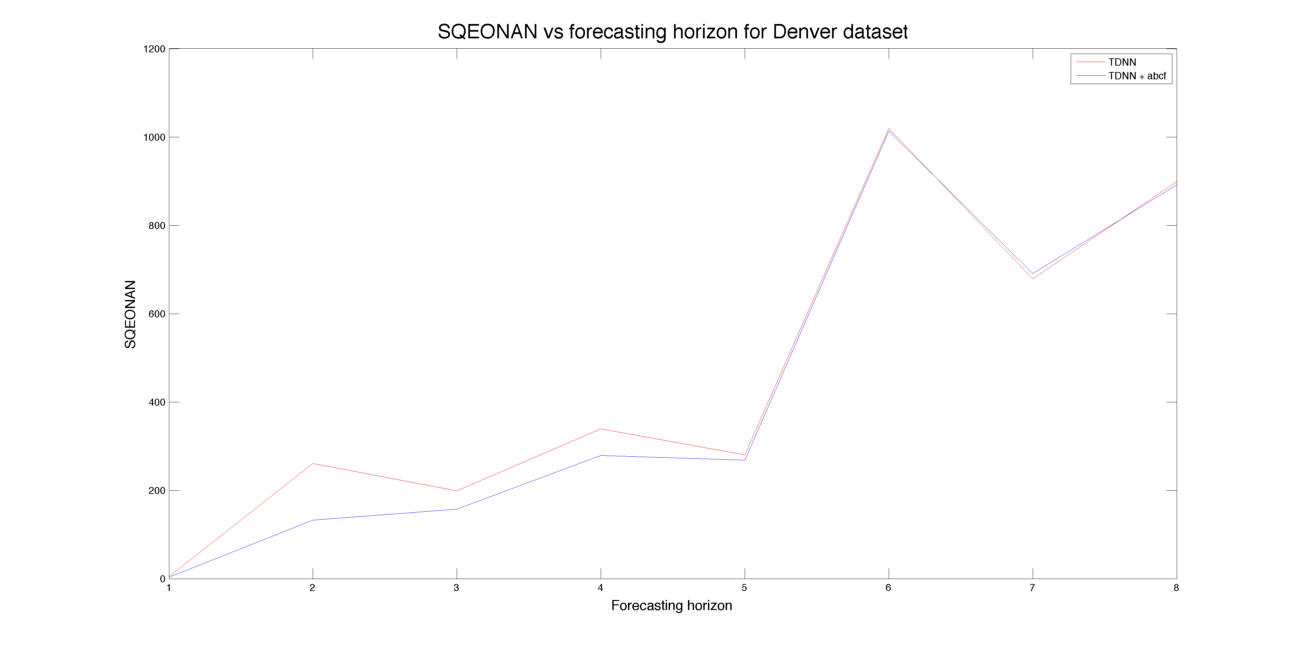
\includegraphics[width=0.4\textwidth]{sqe_denver_tdnn.png}
		}
	\end{center}
	\caption{Results for the four base forecasting algorithms for the Denver dataset and the improvements to SQEONAN from using our ABCF algorithm}
	\label{fig:sqe_denver_results}
\end{figure}

\newpage

%%%%%%%%%%%%%%%%%%%%%%%%%%%%%%%%%%%%%%%%%%%%%%%%%
%RMSE Results per forecaster
%%%%%%%%%%%%%%%%%%%%%%%%%%%%%%%%%%%%%%%%%%%%%%%%%
%merl
\begin{figure}[!h]
	\begin{center}
		\subfigure[] {
			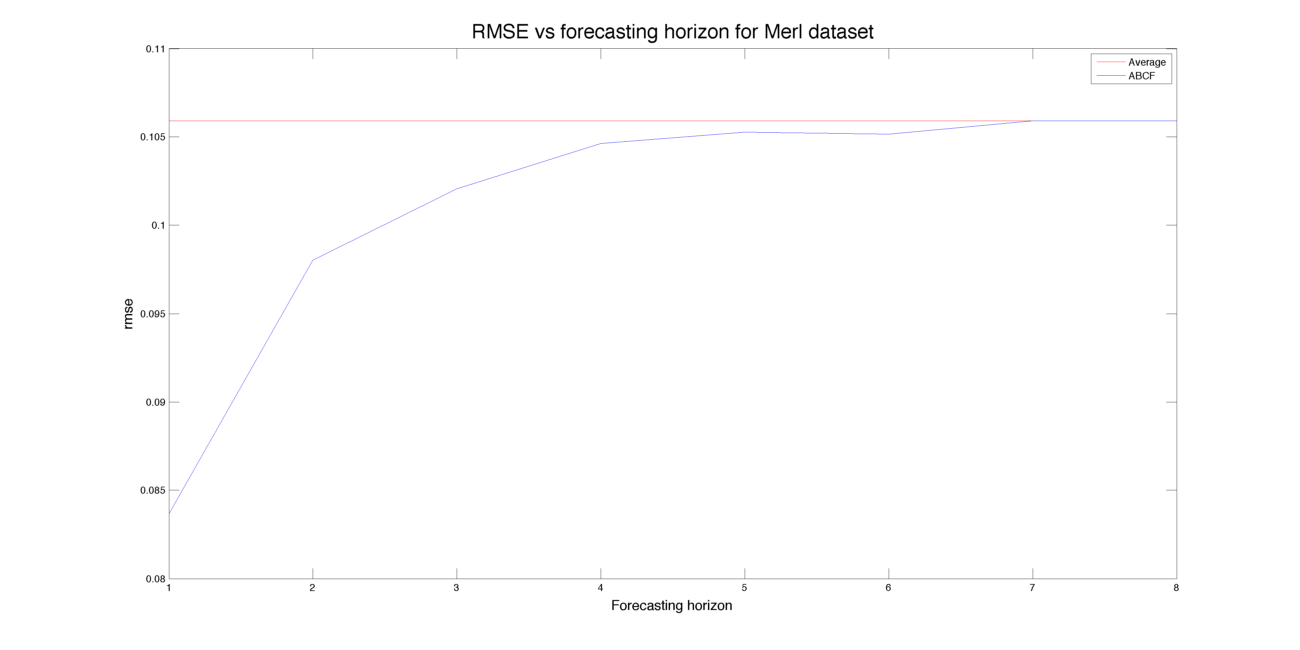
\includegraphics[width=0.4\textwidth]{rmse_merl_avg.png}
		}
		\subfigure[] {
			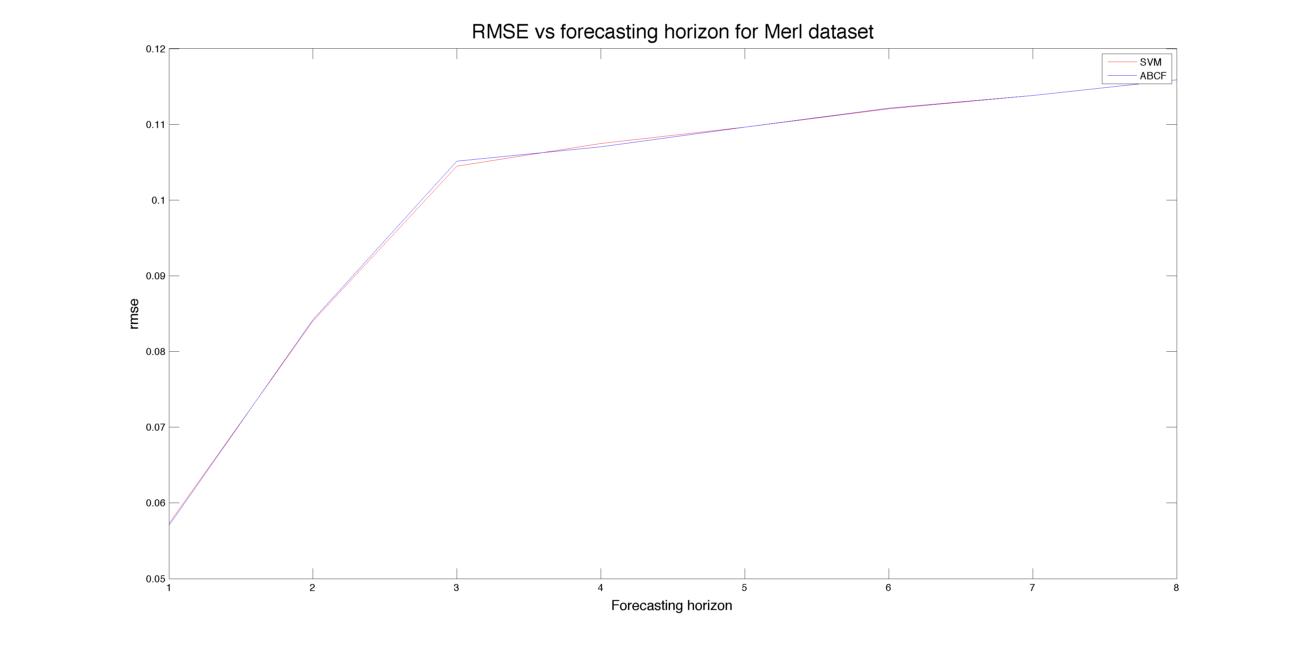
\includegraphics[width=0.4\textwidth]{rmse_merl_svm.png}
		} \\
		\subfigure[] {
			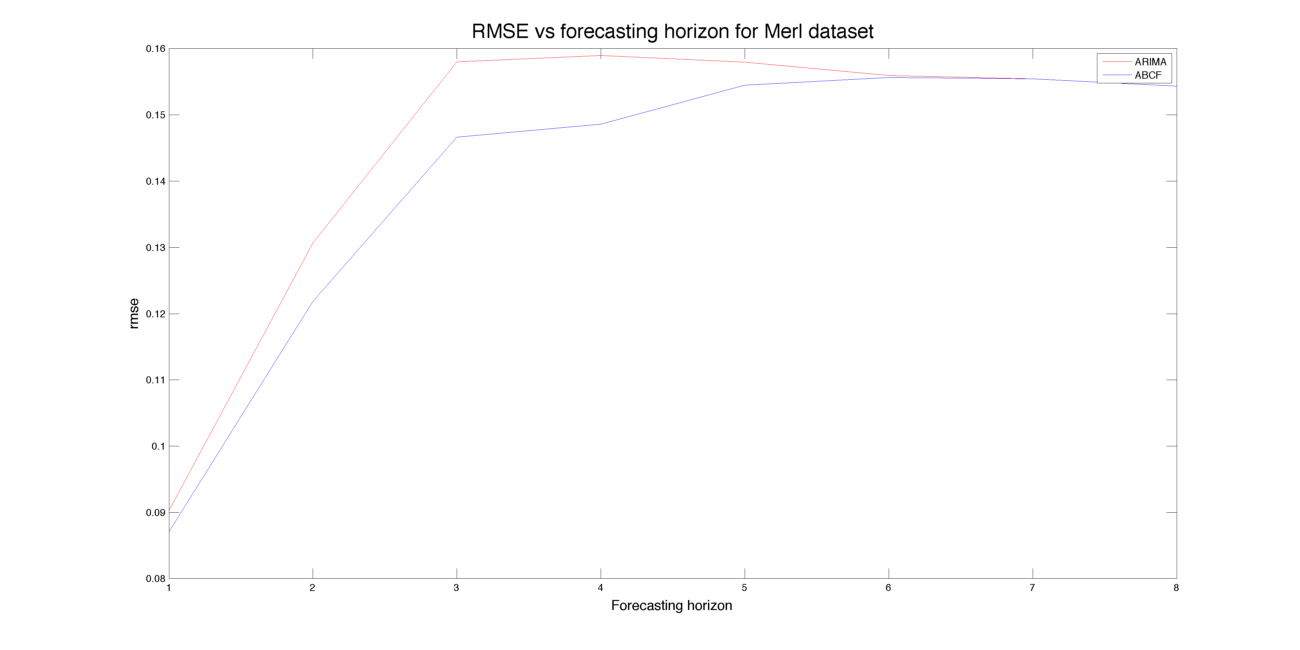
\includegraphics[width=0.4\textwidth]{rmse_merl_arima.png}
		}
		\subfigure[] {
			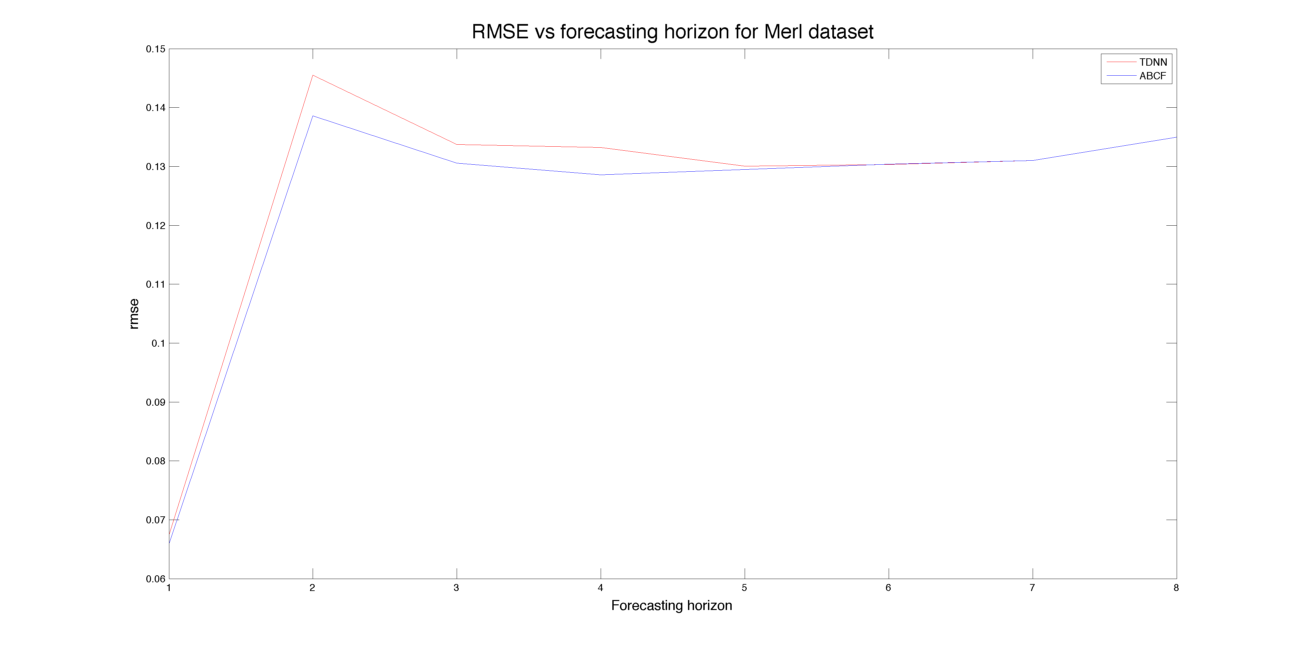
\includegraphics[width=0.4\textwidth]{rmse_merl_tdnn.png}
		}
	\end{center}
	\caption{Results for the four base forecasting algorithms for the MERL dataset and the improvements to RMSE from using our ABCF algorithm}
	\label{fig:rmse_merl_results}
\end{figure}

%brown
\begin{figure}[!h]
	\begin{center}
		\subfigure[] {
			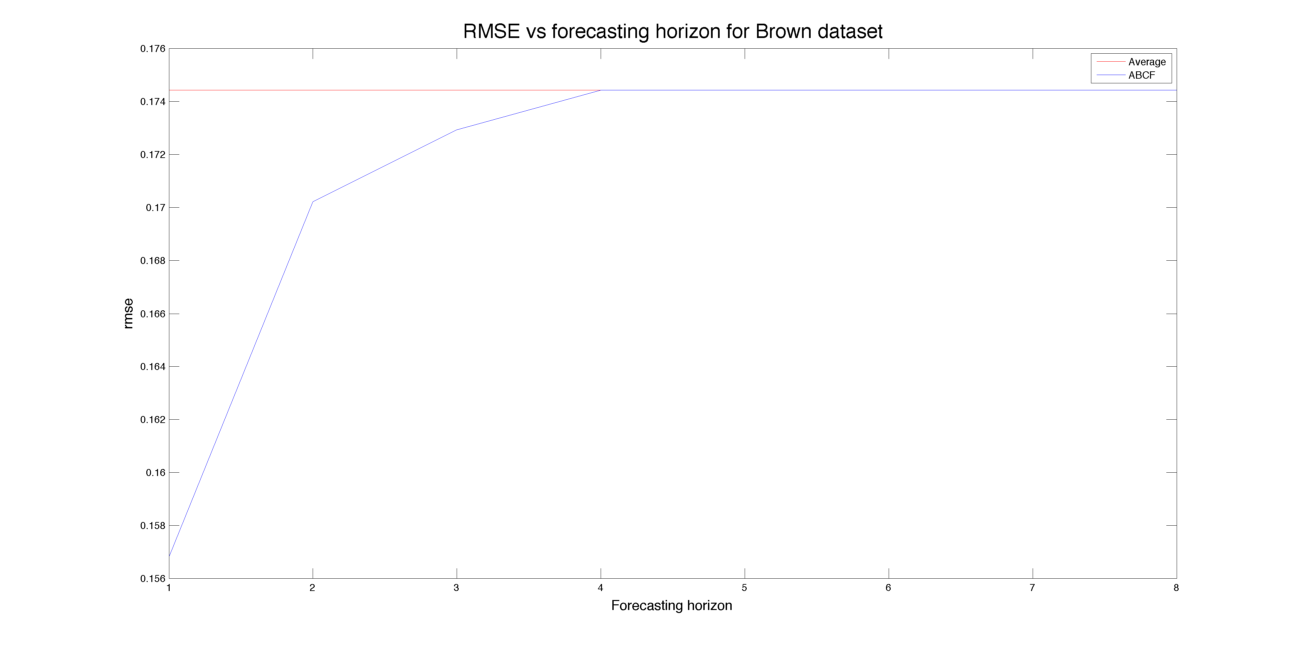
\includegraphics[width=0.4\textwidth]{rmse_brown_avg.png}
		}
		\subfigure[] {
			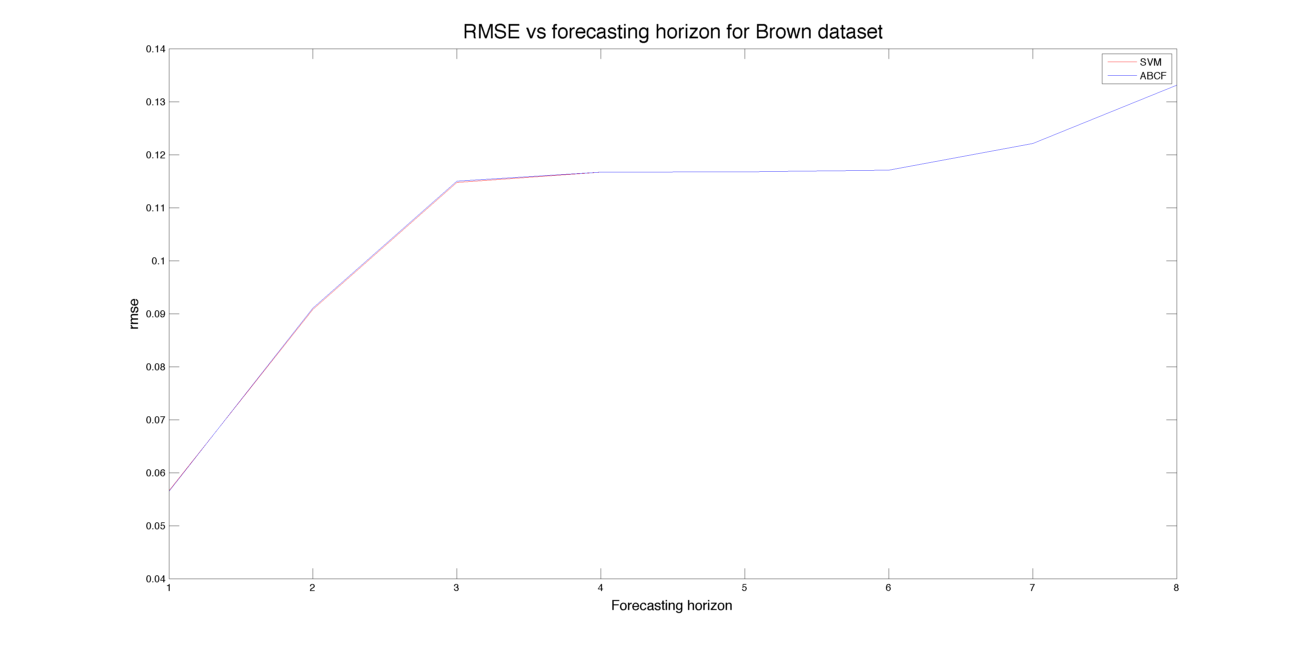
\includegraphics[width=0.4\textwidth]{rmse_brown_svm.png}
		} \\
		\subfigure[] {
			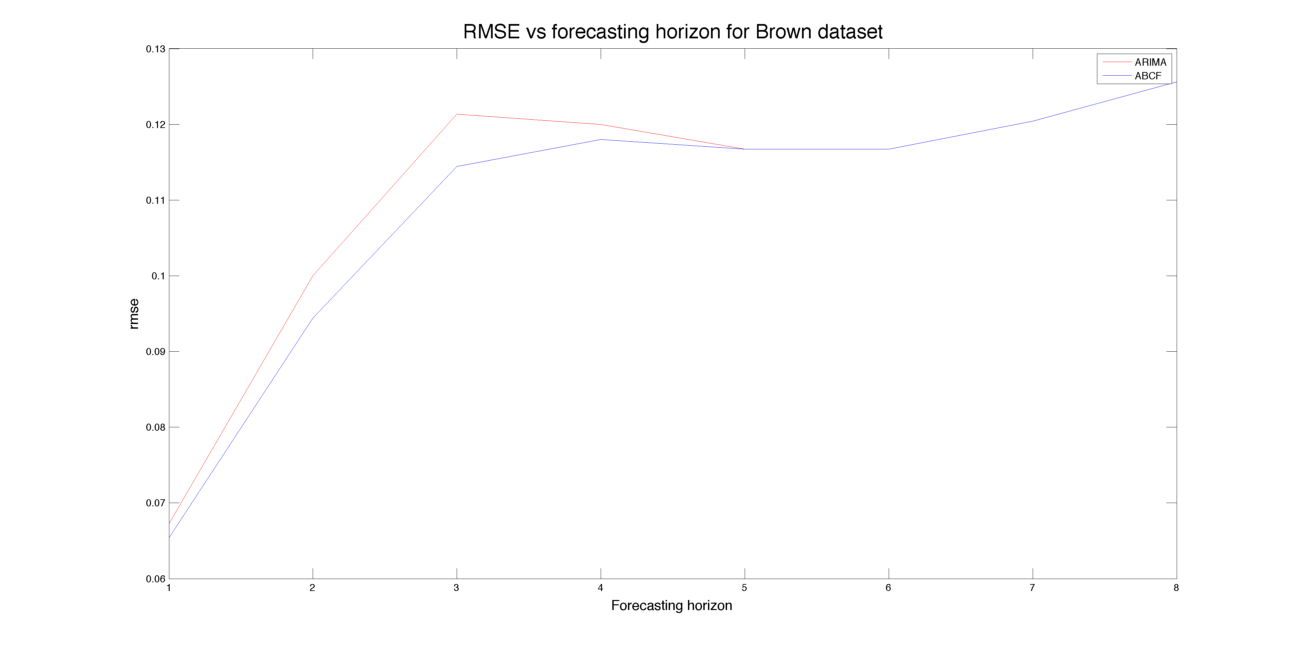
\includegraphics[width=0.4\textwidth]{rmse_brown_arima.png}
		}
		\subfigure[] {
			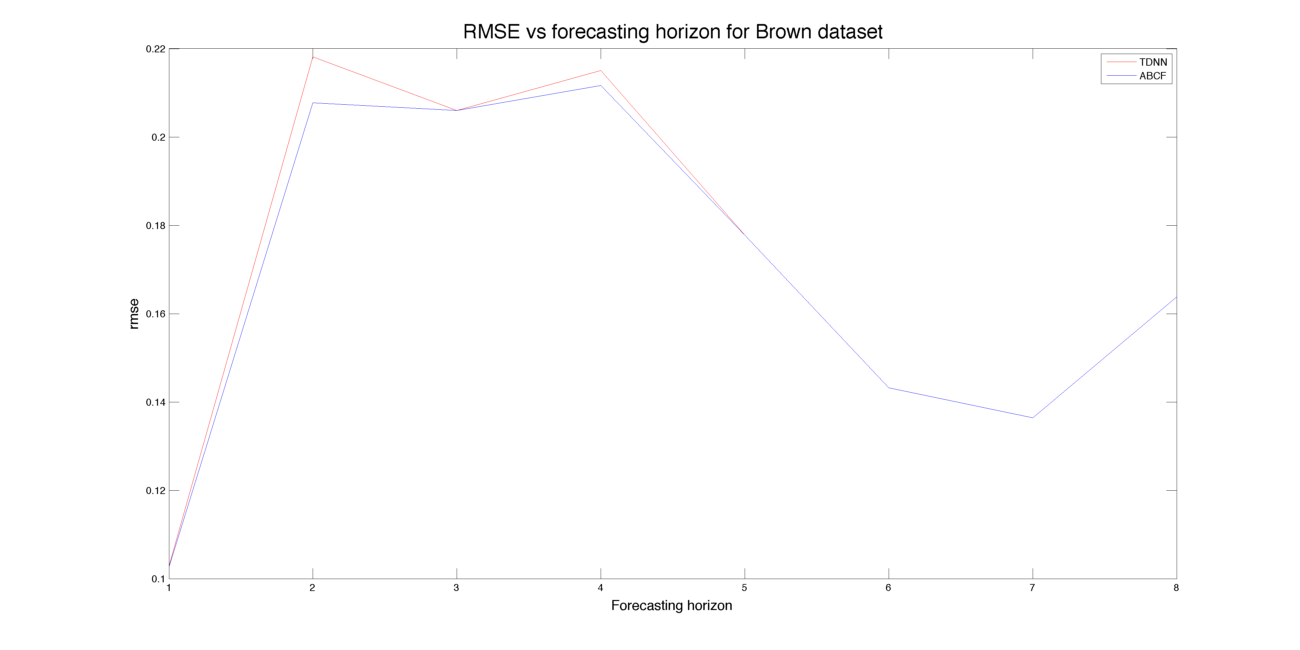
\includegraphics[width=0.4\textwidth]{rmse_brown_tdnn.png}
		}
	\end{center}
	\caption{Results for the four base forecasting algorithms for the Brown Hall dataset and the improvements to RMSE from using our ABCF algorithm}
	\label{fig:rmse_brown_results}
\end{figure}

%denver
\begin{figure}[!h]
	\begin{center}
		\subfigure[] {
			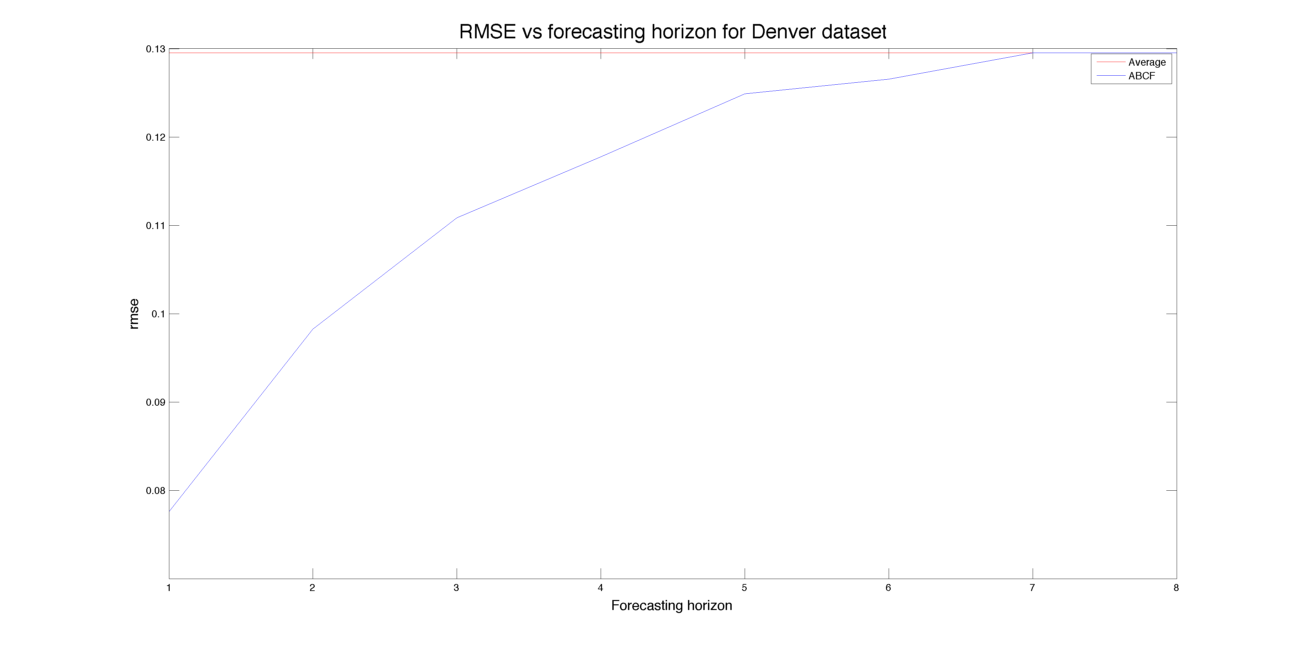
\includegraphics[width=0.4\textwidth]{rmse_denver_avg.png}
		}
		\subfigure[] {
			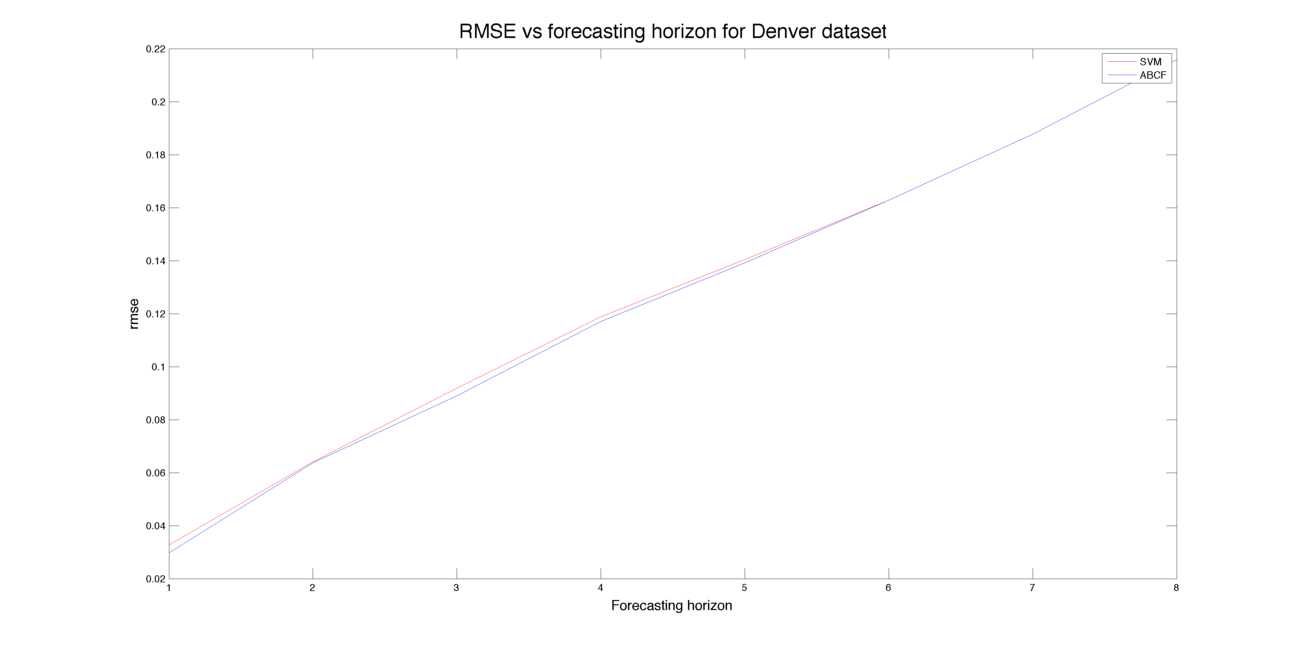
\includegraphics[width=0.4\textwidth]{rmse_denver_svm.png}
		} \\
		\subfigure[] {
			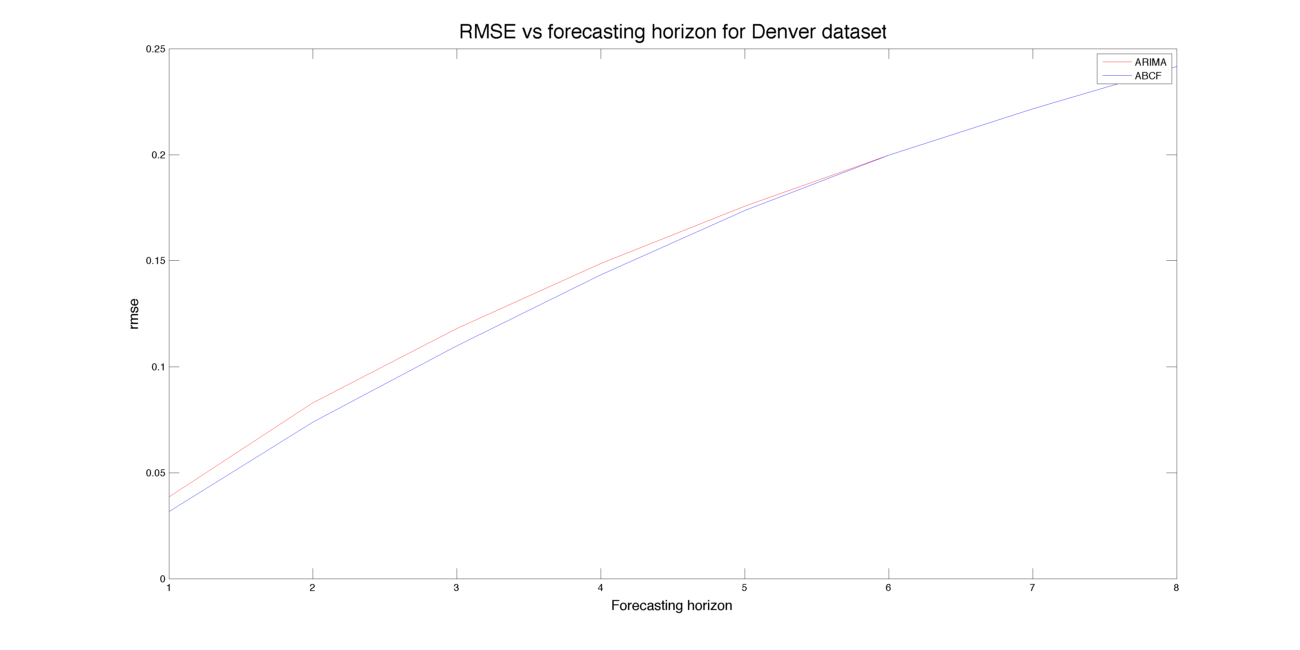
\includegraphics[width=0.4\textwidth]{rmse_denver_arima.png}
		}
		\subfigure[] {
			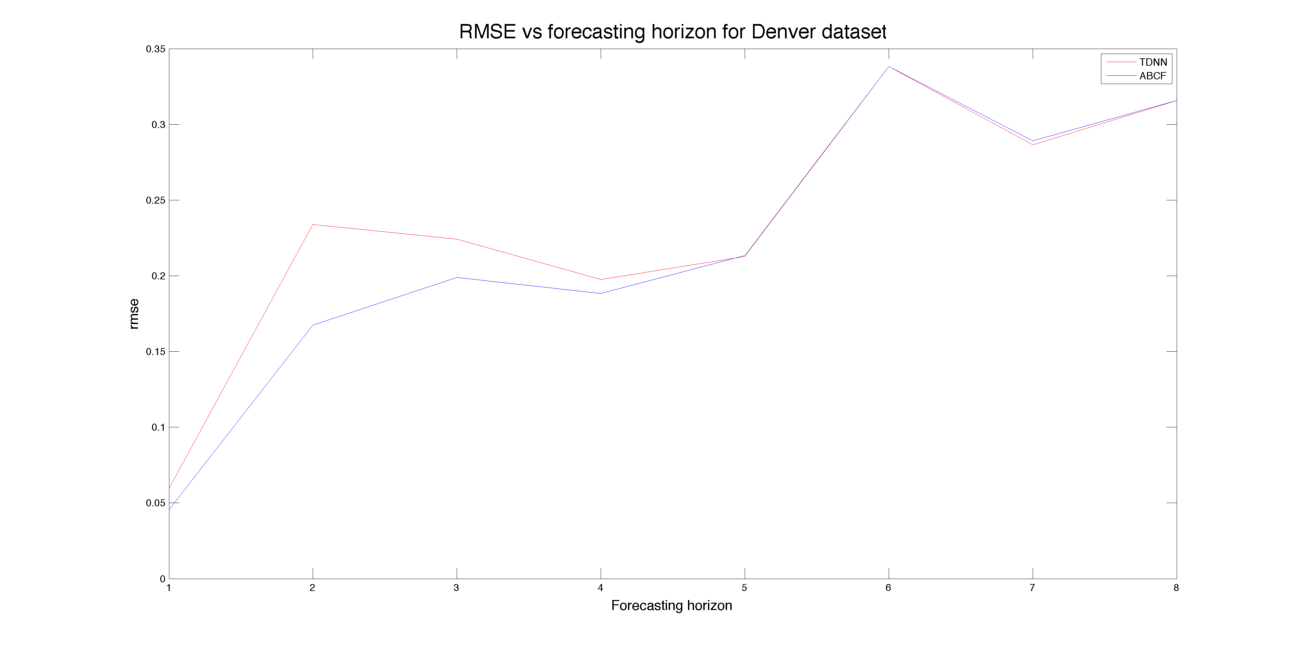
\includegraphics[width=0.4\textwidth]{rmse_denver_tdnn.png}
		}
	\end{center}
	\caption{Results for the four base forecasting algorithms for the Denver dataset and the improvements to RMSE from using our ABCF algorithm}
	\label{fig:rmse_denver_results}
\end{figure}

\newpage

%%%%%%%%%%%%%%%%%%%%%%%%%%%%%%%%%%%%%%%%%%%%%%%%%
%MASE Results per forecaster
%%%%%%%%%%%%%%%%%%%%%%%%%%%%%%%%%%%%%%%%%%%%%%%%%
%merl
\begin{figure}[!h]
	\begin{center}
		\subfigure[] {
			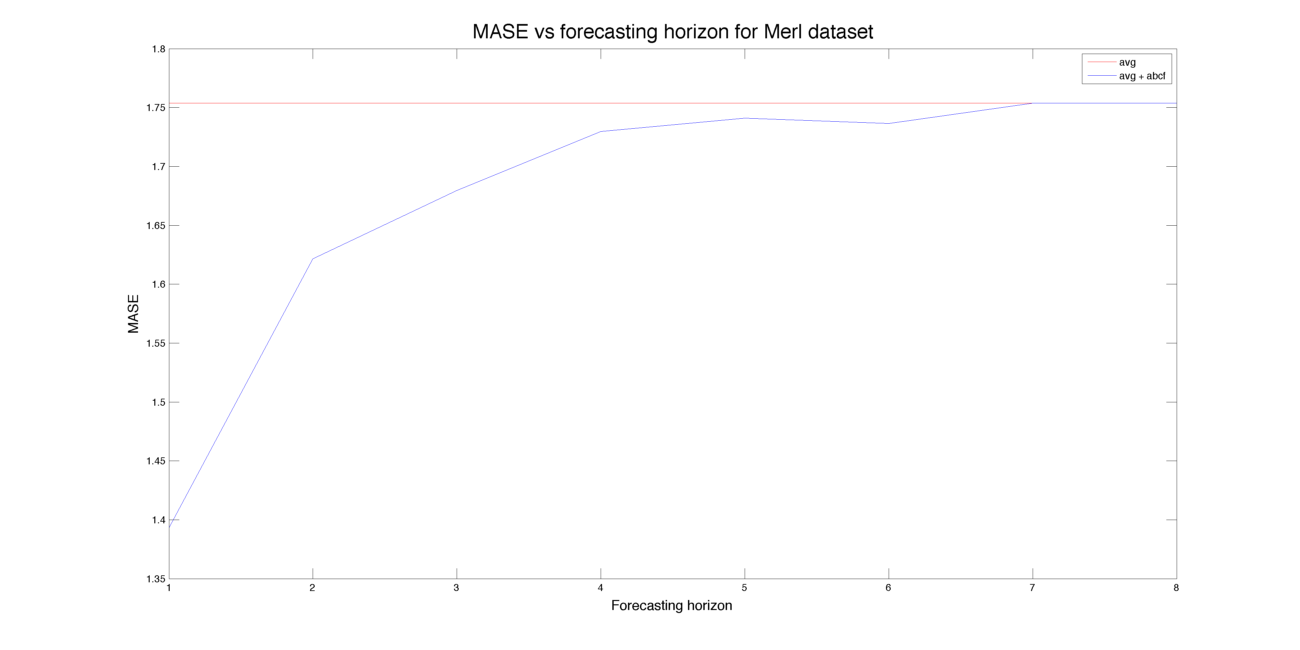
\includegraphics[width=0.4\textwidth]{mase_Merl_avg.png}
		}
		\subfigure[] {
			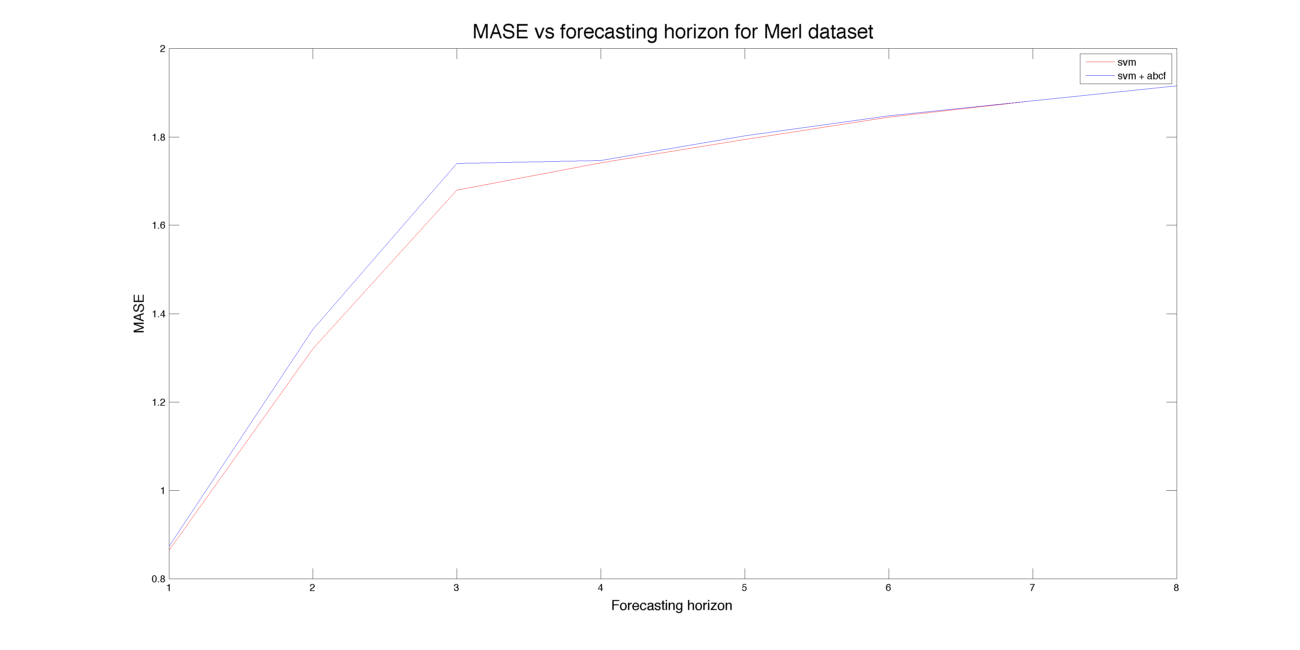
\includegraphics[width=0.4\textwidth]{mase_Merl_svm.png}
		} \\
		\subfigure[] {
			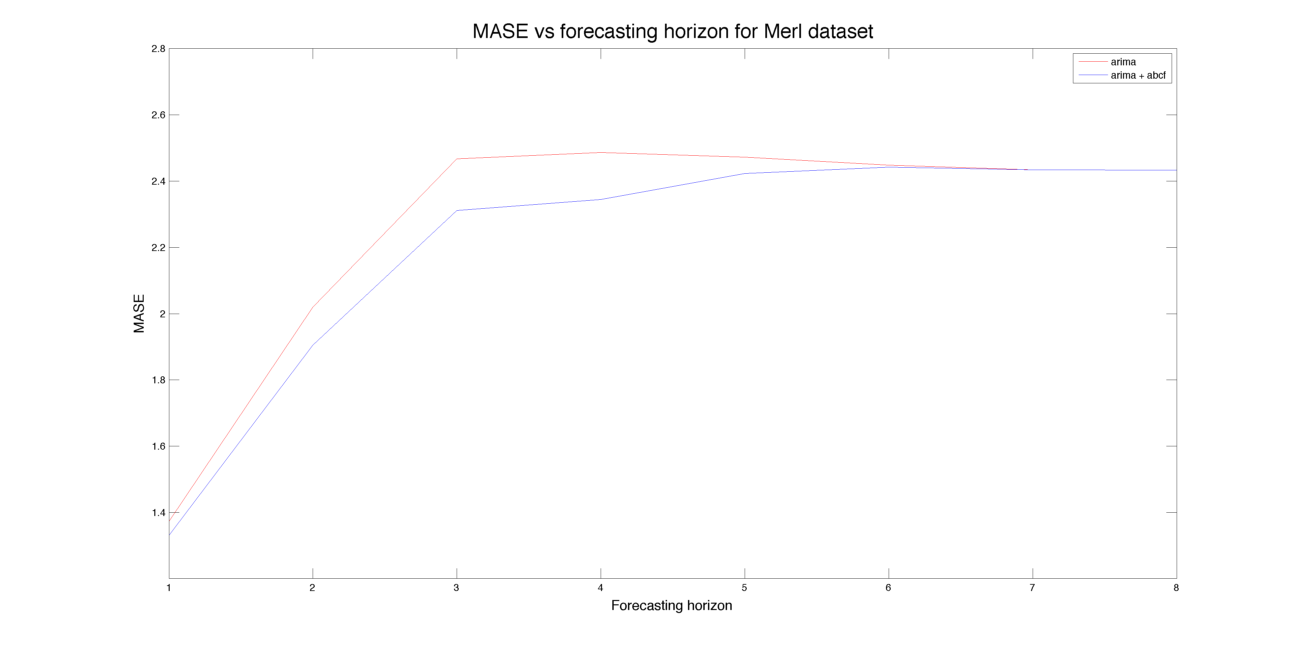
\includegraphics[width=0.4\textwidth]{mase_Merl_arima.png}
		}
		\subfigure[] {
			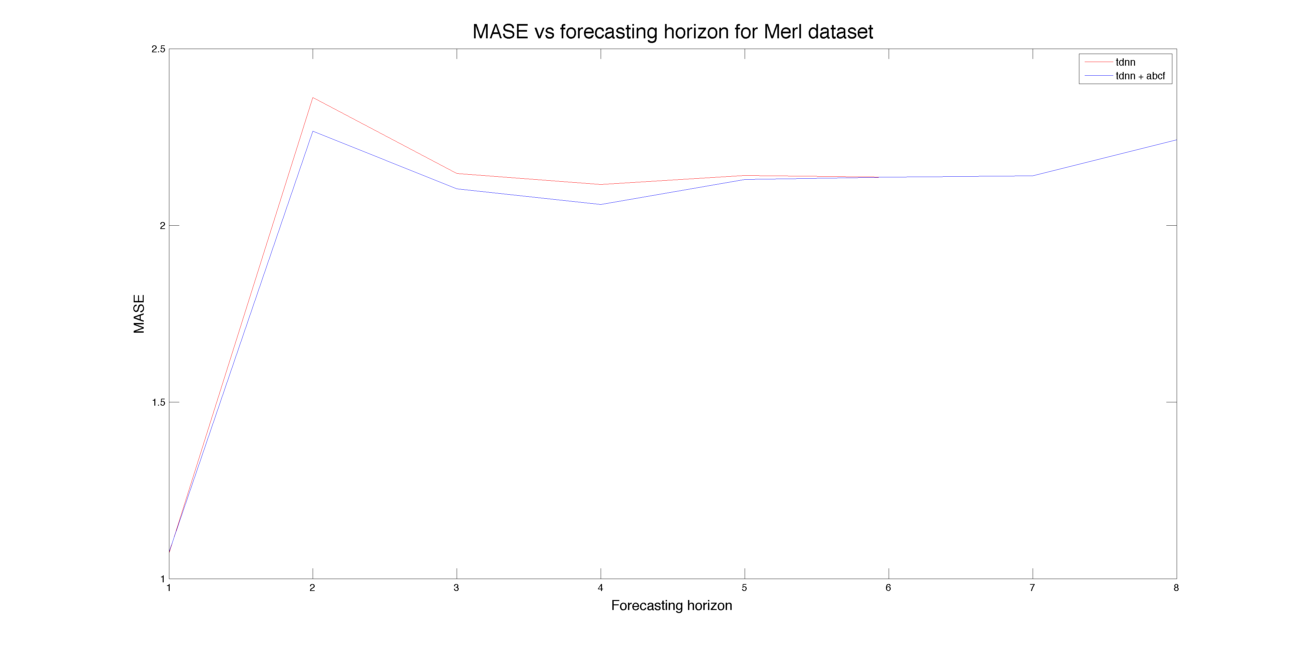
\includegraphics[width=0.4\textwidth]{mase_Merl_tdnn.png}
		}
	\end{center}
	\caption{Results for the four base forecasting algorithms for the MERL dataset and the improvements to MASE from using our ABCF algorithm}
	\label{fig:mase_merl_results}
\end{figure}

%brown
\begin{figure}[!b]
	\begin{center}
		\subfigure[] {
			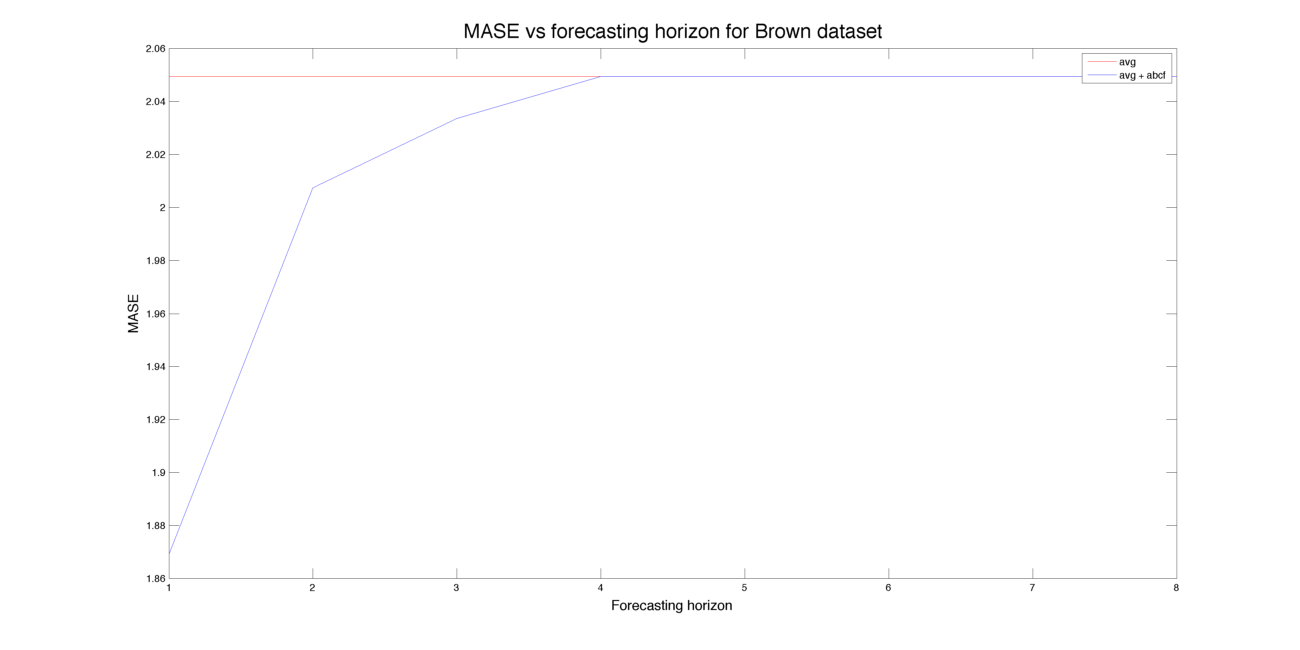
\includegraphics[width=0.4\textwidth]{mase_Brown_avg.png}
		}
		\subfigure[] {
			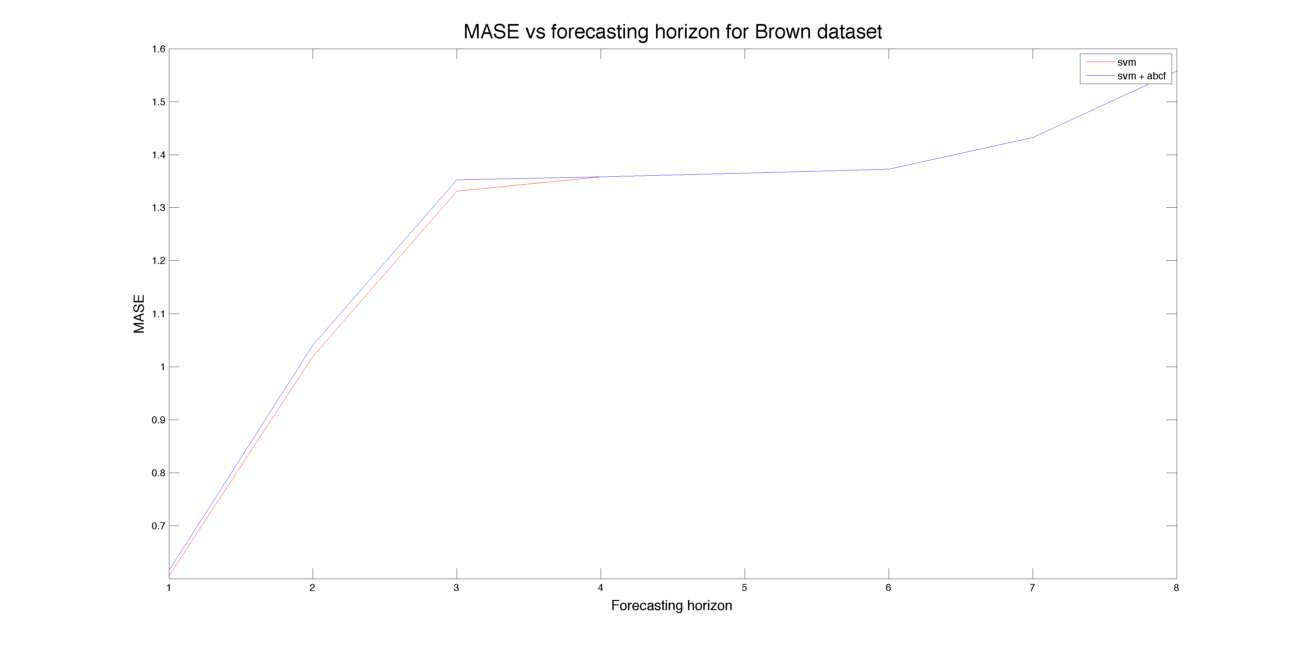
\includegraphics[width=0.4\textwidth]{mase_Brown_svm.png}
		} \\
		\subfigure[] {
			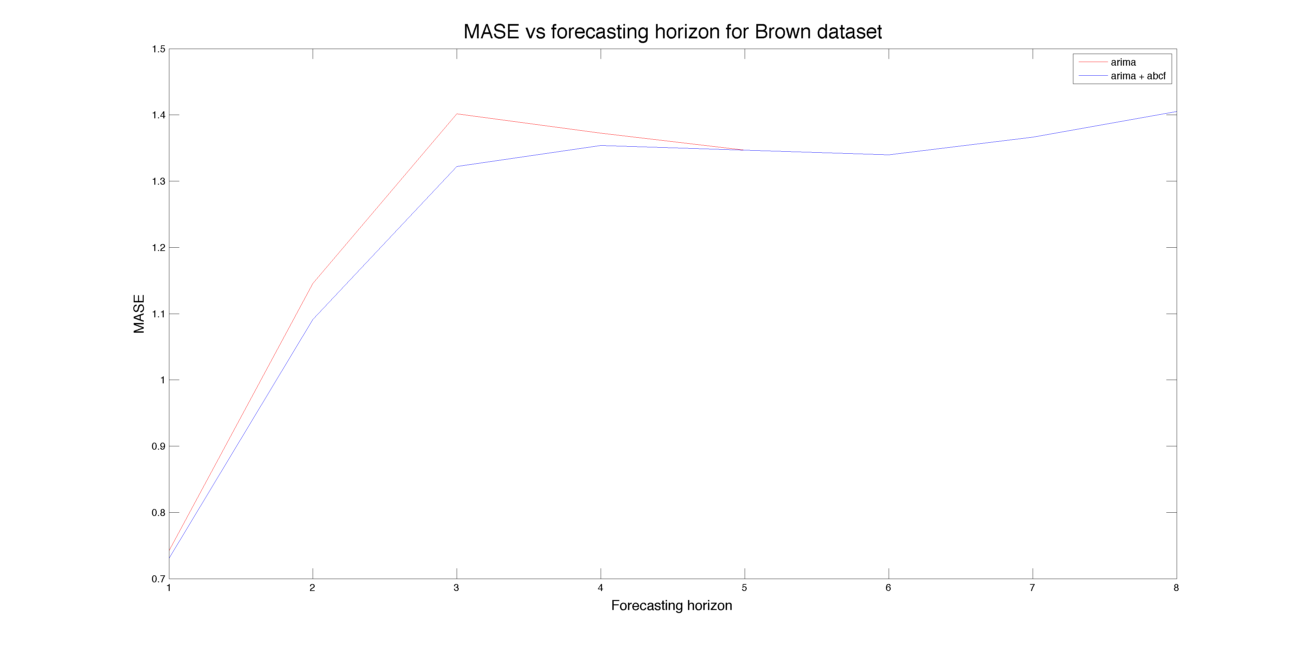
\includegraphics[width=0.4\textwidth]{mase_Brown_arima.png}
		}
		\subfigure[] {
			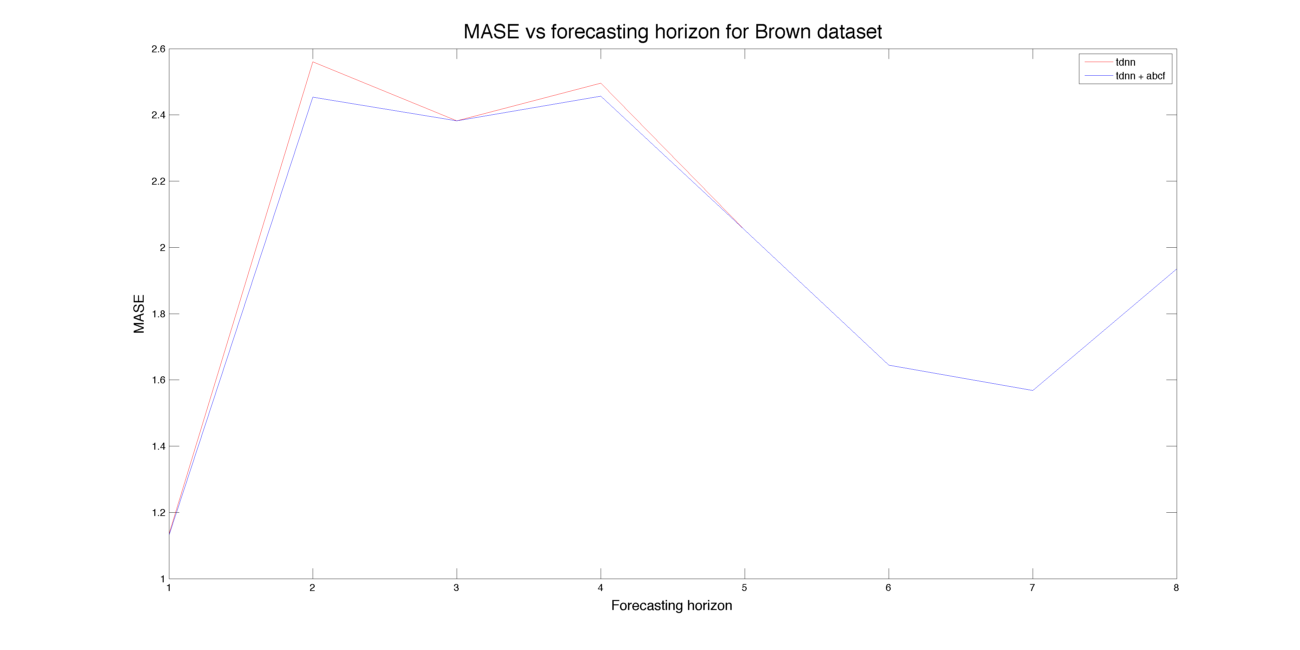
\includegraphics[width=0.4\textwidth]{mase_Brown_tdnn.png}
		}
	\end{center}
	\caption{Results for the four base forecasting algorithms for the Brown Hall dataset and the improvements to MASE from using our ABCF algorithm}
	\label{fig:mase_brown_results}
\end{figure}

%denver
\begin{figure}[!t]
	\begin{center}
		\subfigure[] {
			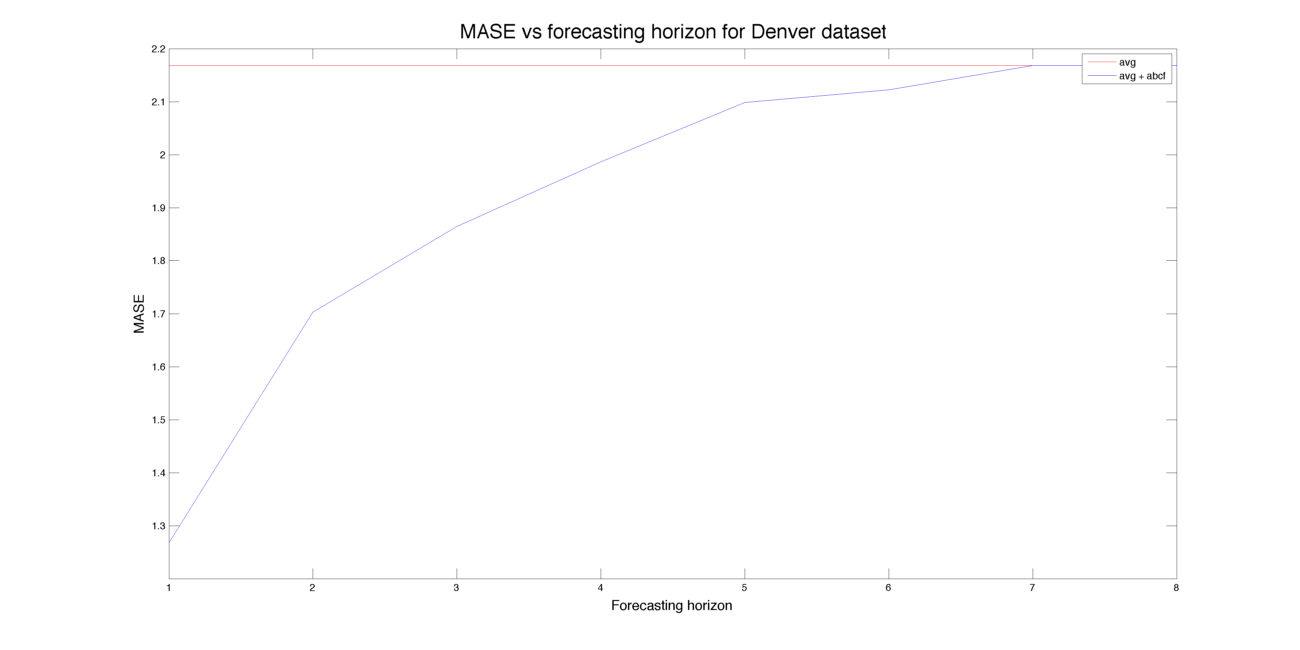
\includegraphics[width=0.4\textwidth]{mase_Denver_avg.png}
		}
		\subfigure[] {
			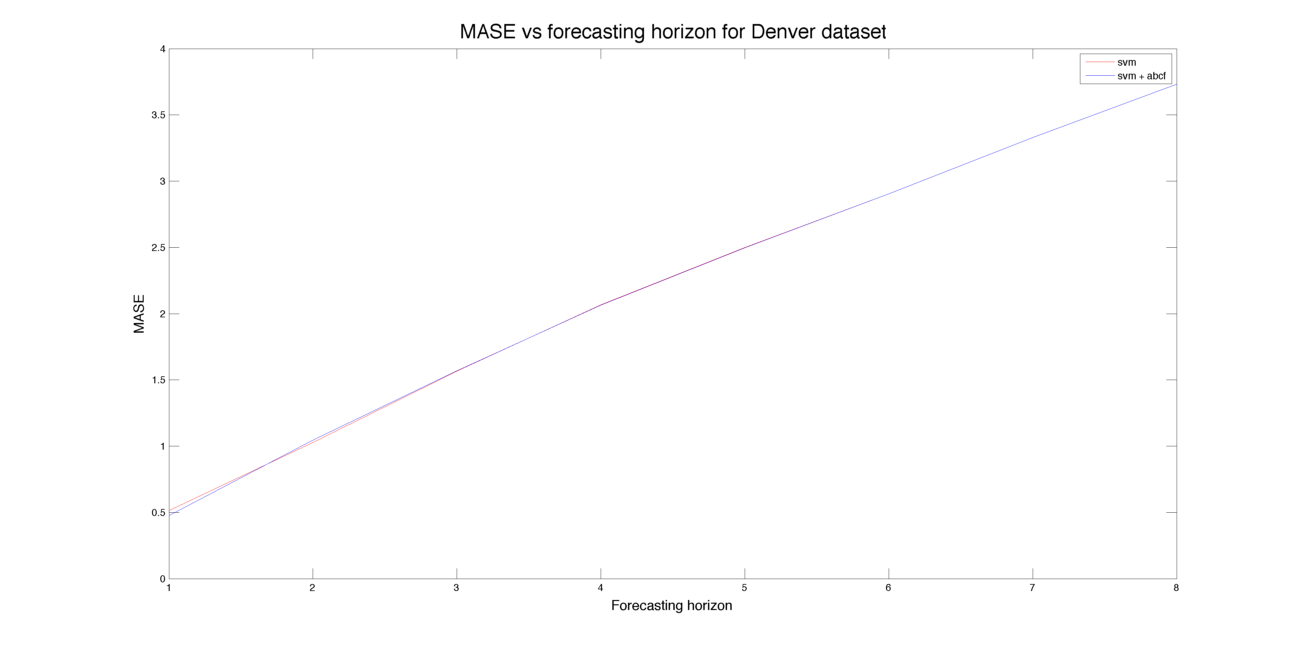
\includegraphics[width=0.4\textwidth]{mase_Denver_svm.png}
		} \\
		\subfigure[] {
			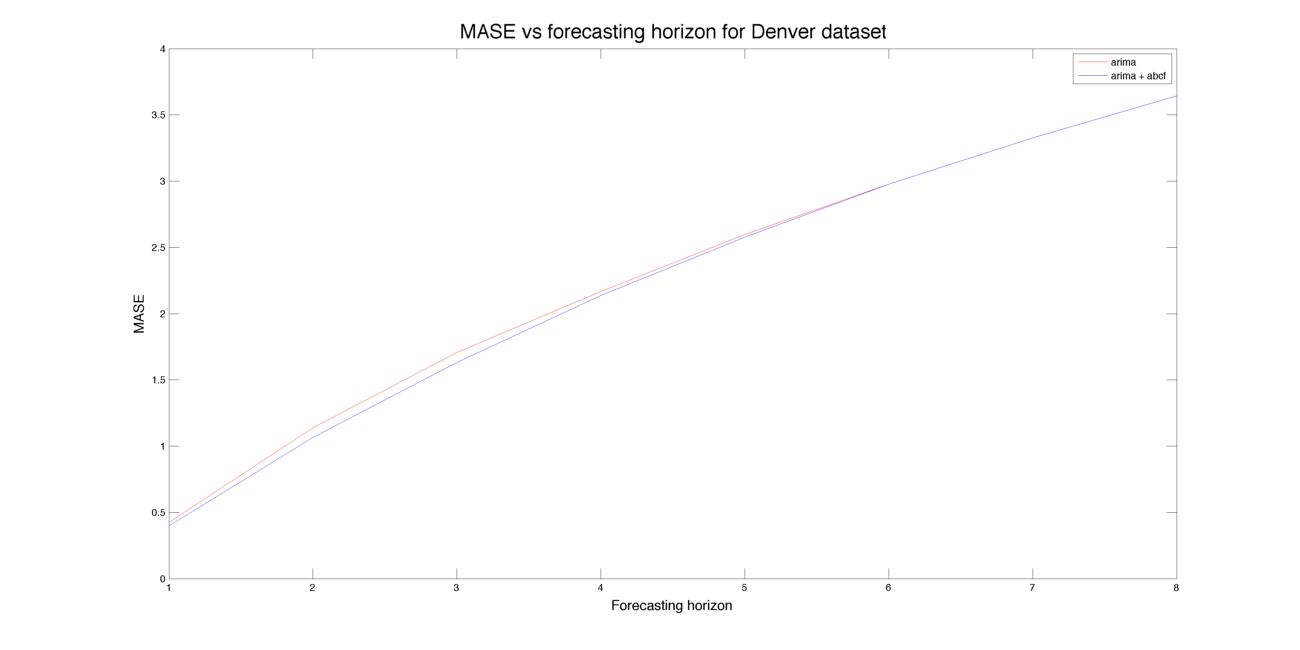
\includegraphics[width=0.4\textwidth]{mase_Denver_arima.png}
		}
		\subfigure[] {
			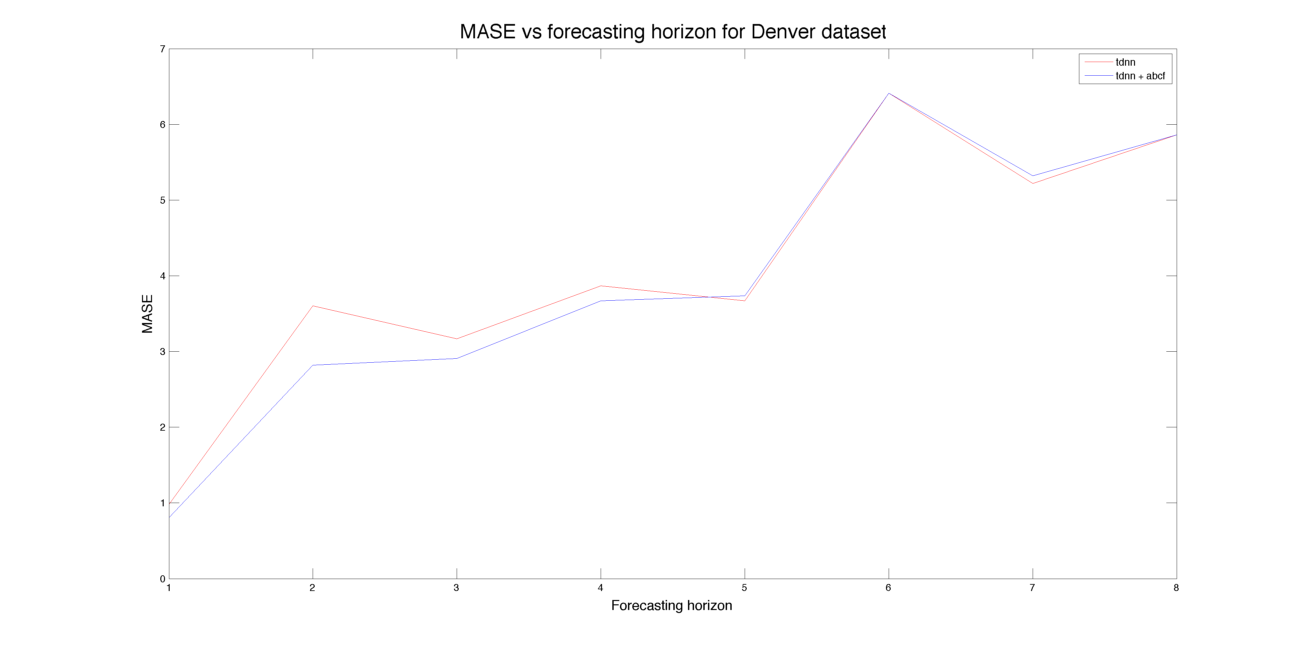
\includegraphics[width=0.4\textwidth]{mase_Denver_tdnn.png}
		}
	\end{center}
	\caption{Results for the four base forecasting algorithms for the Denver dataset and the improvements to MASE from using our ABCF algorithm}
	\label{fig:mase_denver_results}
\end{figure}


%%%%%%%%%%%%%%%%%%%%%%%%%%%%%%%%%%%%%%%%%%%%%%%%%
%RMSE Results per DATASET
%%%%%%%%%%%%%%%%%%%%%%%%%%%%%%%%%%%%%%%%%%%%%%%%%
\begin{figure}[!b]
	\begin{center}
		\subfigure[] {
			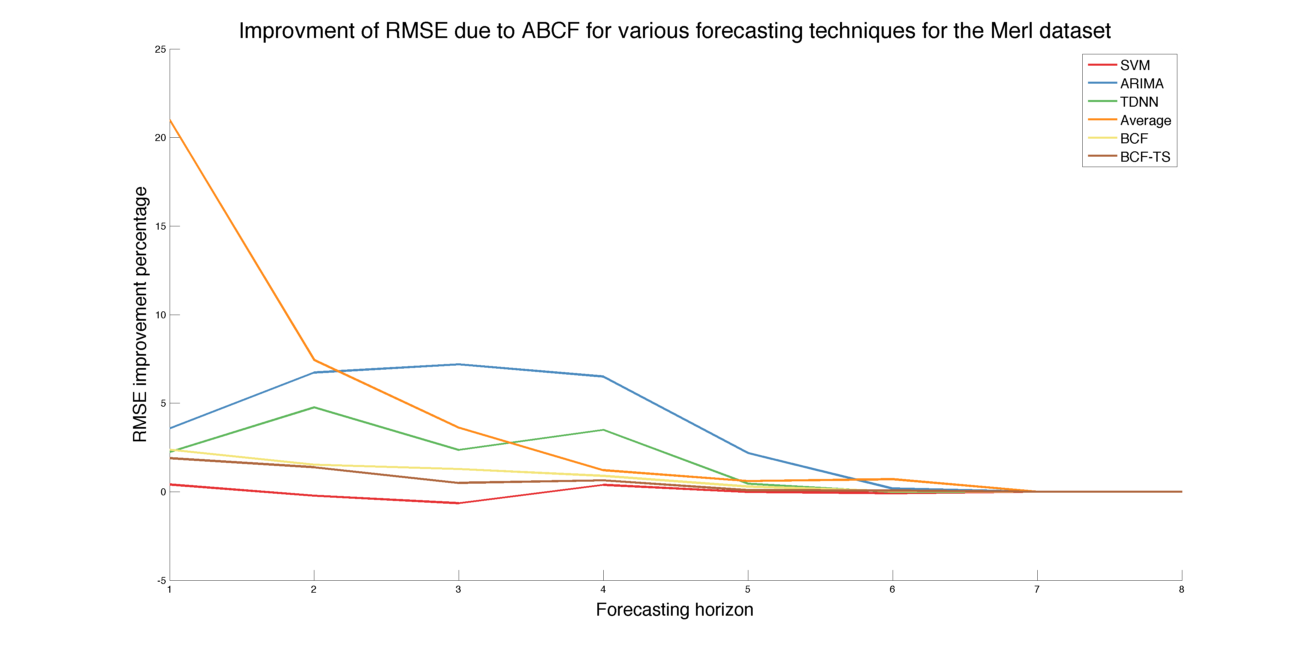
\includegraphics[width=0.49\textwidth]{rmse_improvement_for_each_forecaster_for_Merl.png}
		}
		\subfigure[] {
			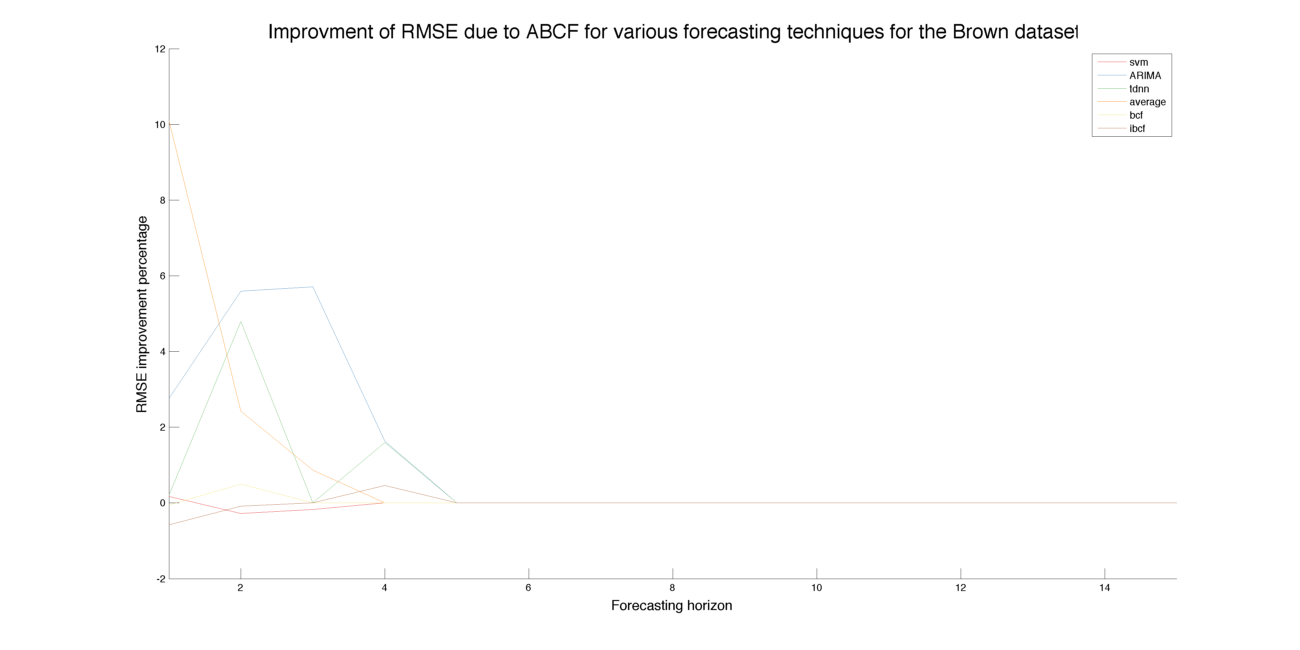
\includegraphics[width=0.49\textwidth]{rmse_improvement_for_each_forecaster_for_Brown.png}
		} \\
		\subfigure[] {
			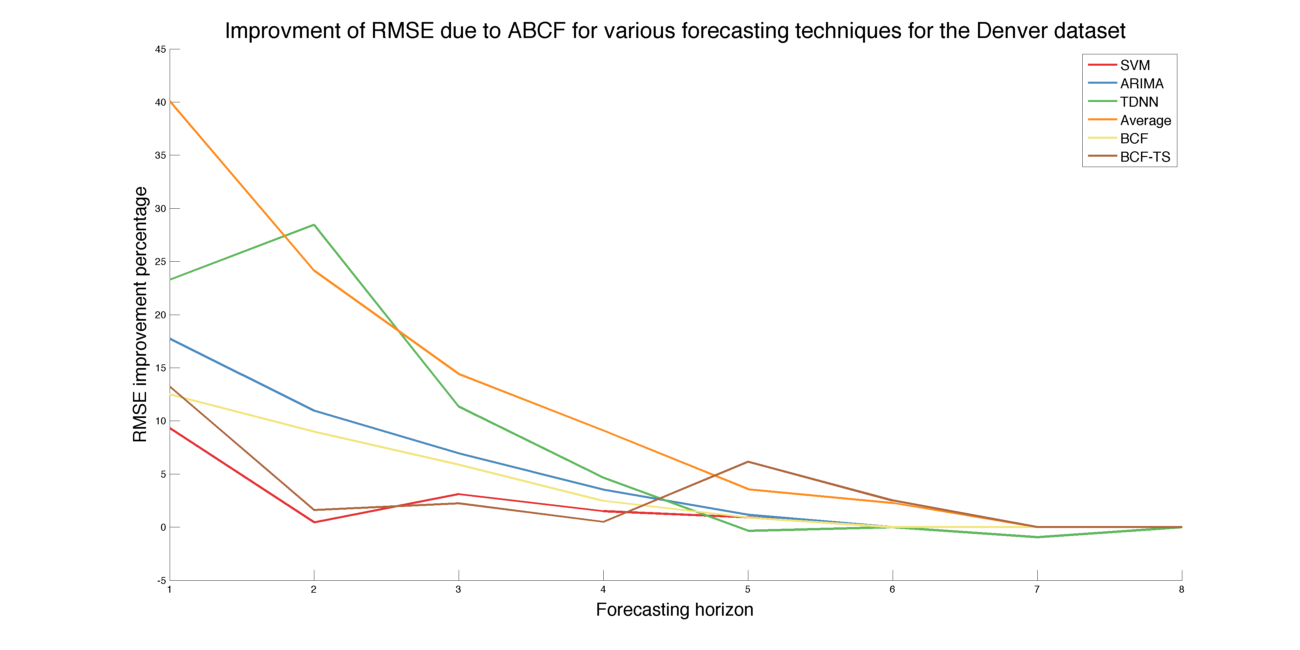
\includegraphics[width=0.49\textwidth]{rmse_improvement_for_each_forecaster_for_Denver.png}
		}
	\end{center}
	\caption{Percentage improvement to RMSE due to application of ABCF}
	\label{fig:rmse_improvement_dataset}
\end{figure}


%%%%%%%%%%%%%%%%%%%%%%%%%%%%%%%%%%%%%%%%%%%%%%%%%
%Reference appendix
%%%%%%%%%%%%%%%%%%%%%%%%%%%%%%%%%%%%%%%%%%%%%%%%%
\appendix{Figure references}\label{app:references}
This thesis was far too long in coming and far to full of various figures that do not have nice references.  
	\footnote{This footnote is simply to reference all of the unreferenced images.  Enjoy.
		\ref{fig:sqe_merl_results},
		\ref{fig:sqe_brown_results},
		\ref{fig:sqe_denver_results},
		\ref{fig:rmse_merl_results},
		\ref{fig:rmse_brown_results},
		\ref{fig:rmse_denver_results},
		\ref{fig:mase_merl_results},
		\ref{fig:mase_brown_results},
		\ref{fig:mase_denver_results},
		\ref{fig:rmse_improvement_dataset},
	}